
%%%%%%%%%%%%%%%%%%%%%%%%%%%%%%%%%%%%
% Tables
%%%%%%%%%%%%%%%%%%%%%%%%%%%%%%%%%%%%
\begin{table}[H]
\centering
\caption{CPS Summary Statistics \label{tab:sumstat1}}
\centering
\begin{threeparttable}
\begin{tabular}[t]{lcccc}
\toprule
\multicolumn{1}{c}{ } & \multicolumn{1}{c}{\textbf{Overall}} & \multicolumn{3}{c}{\textbf{By Generation}} \\
\cmidrule(l{3pt}r{3pt}){2-2} \cmidrule(l{3pt}r{3pt}){3-5}
\textbf{Characteristic} & \makecell[c]{\textbf{All Sample} \\N = 318,404} & \makecell[c]{\textbf{First} \\N=40,033} & \makecell[c]{\textbf{Second} \\N=199,294} & \makecell[c]{\textbf{Third} \\N=79,077}\\
\midrule
Female & 0.49 & 0.53 & 0.49 & 0.49\\
Asian & 0.65 & 0.96 & 0.73 & 0.31\\
Age & 8.4 (5.1) & 10.9 (4.5) & 8.3 (5.1) & 7.7 (5.0)\\
College Graduate:\ \ 	 Father & 0.52 & 0.59 & 0.52 & 0.50\\
College Graduate:\ \ 	 Mother & 0.52 & 0.56 & 0.51 & 0.52\\
Total Family Income\ \ 	 (1999 dollars) & 87,031 (84,797) & 75,815 (74,489) & 88,295 (88,411) & 89,436 (80,051)\\
\bottomrule
\end{tabular}
\begin{tablenotes}
\item[1] The samples include children ages 17 and below who live in intact families. First-generation Asian immigrant children that were born in a Asian country. Native-born second-generation Asian immigrant children with at least one parent born in a Asian country. Finally, native-born third generation Asian immigrant children with native-born parents and at least one grand parent born in a Asian country.
\item[2] Data source is the 2004-2021 Current Population Survey.
\end{tablenotes}
\end{threeparttable}
\end{table}



\begin{table}[H]
\centering\centering
\caption{Asian Self-identification by Generation \label{tab:hispbygen}}
\centering
\begin{threeparttable}
\begin{tabular}[t]{>{}lcccc}
\toprule
  & \specialcell{Self-identify \\ as Asian} & \specialcell{Self-identify as \\ non-Asian} & \specialcell{\% Self-identify \\ as Asian} & \specialcell{\% Self-identify \\ as non-Asian}\\
\midrule
\textbf{1st Gen.} & 14,811 & 688 & 0.96 & 0.04\\
\textbf{2nd Gen.} & 58,756 & 21,381 & 0.73 & 0.27\\
\hspace{1em}\textbf{Asian on:} &  &  &  \vphantom{1} & \\
\hspace{1em}\hspace{1em}\textbf{Both Sides} & 49,118 & 1,717 & 0.97 & 0.03\\
\hspace{1em}\hspace{1em}\textbf{One Side} & 9,638 & 19,664 & 0.33 & 0.67\\
\addlinespace
\textbf{3rd Gen.} & 10,394 & 23,048 & 0.31 & 0.69\\
\hspace{1em}\textbf{Asian on:} &  &  &  & \\
\hspace{1em}\hspace{1em}\textbf{Both Sides} & 5,428 & 316 & 0.94 & 0.06\\
\hspace{1em}\hspace{1em}\textbf{One Side} & 3,030 & 9,213 & 0.25 & 0.75\\
\bottomrule
\end{tabular}
\begin{tablenotes}
\item[1] The samples include children ages 17 and below who live in intact families. First-generation Asian immigrant children that were born in a Asian country. Native-born second-generation Asian immigrant children with at least one parent born in a Asian country. Finally, native-born third-generation Asian immigrant children with native-born parents and at least one grandparent born in a Asian country.
\item[2] Data source is the 2004-2021 Current Population Survey.
\end{tablenotes}
\end{threeparttable}
\end{table}


\begin{center}
\begin{figure}[H]
\caption{Bias and Self-reported Asian Identity in the Least and Most Biased Places}

% first
\begin{subfigure}{.9\textwidth}
\caption{Skin Tone Implicit Association Bias Over Time}
\centering
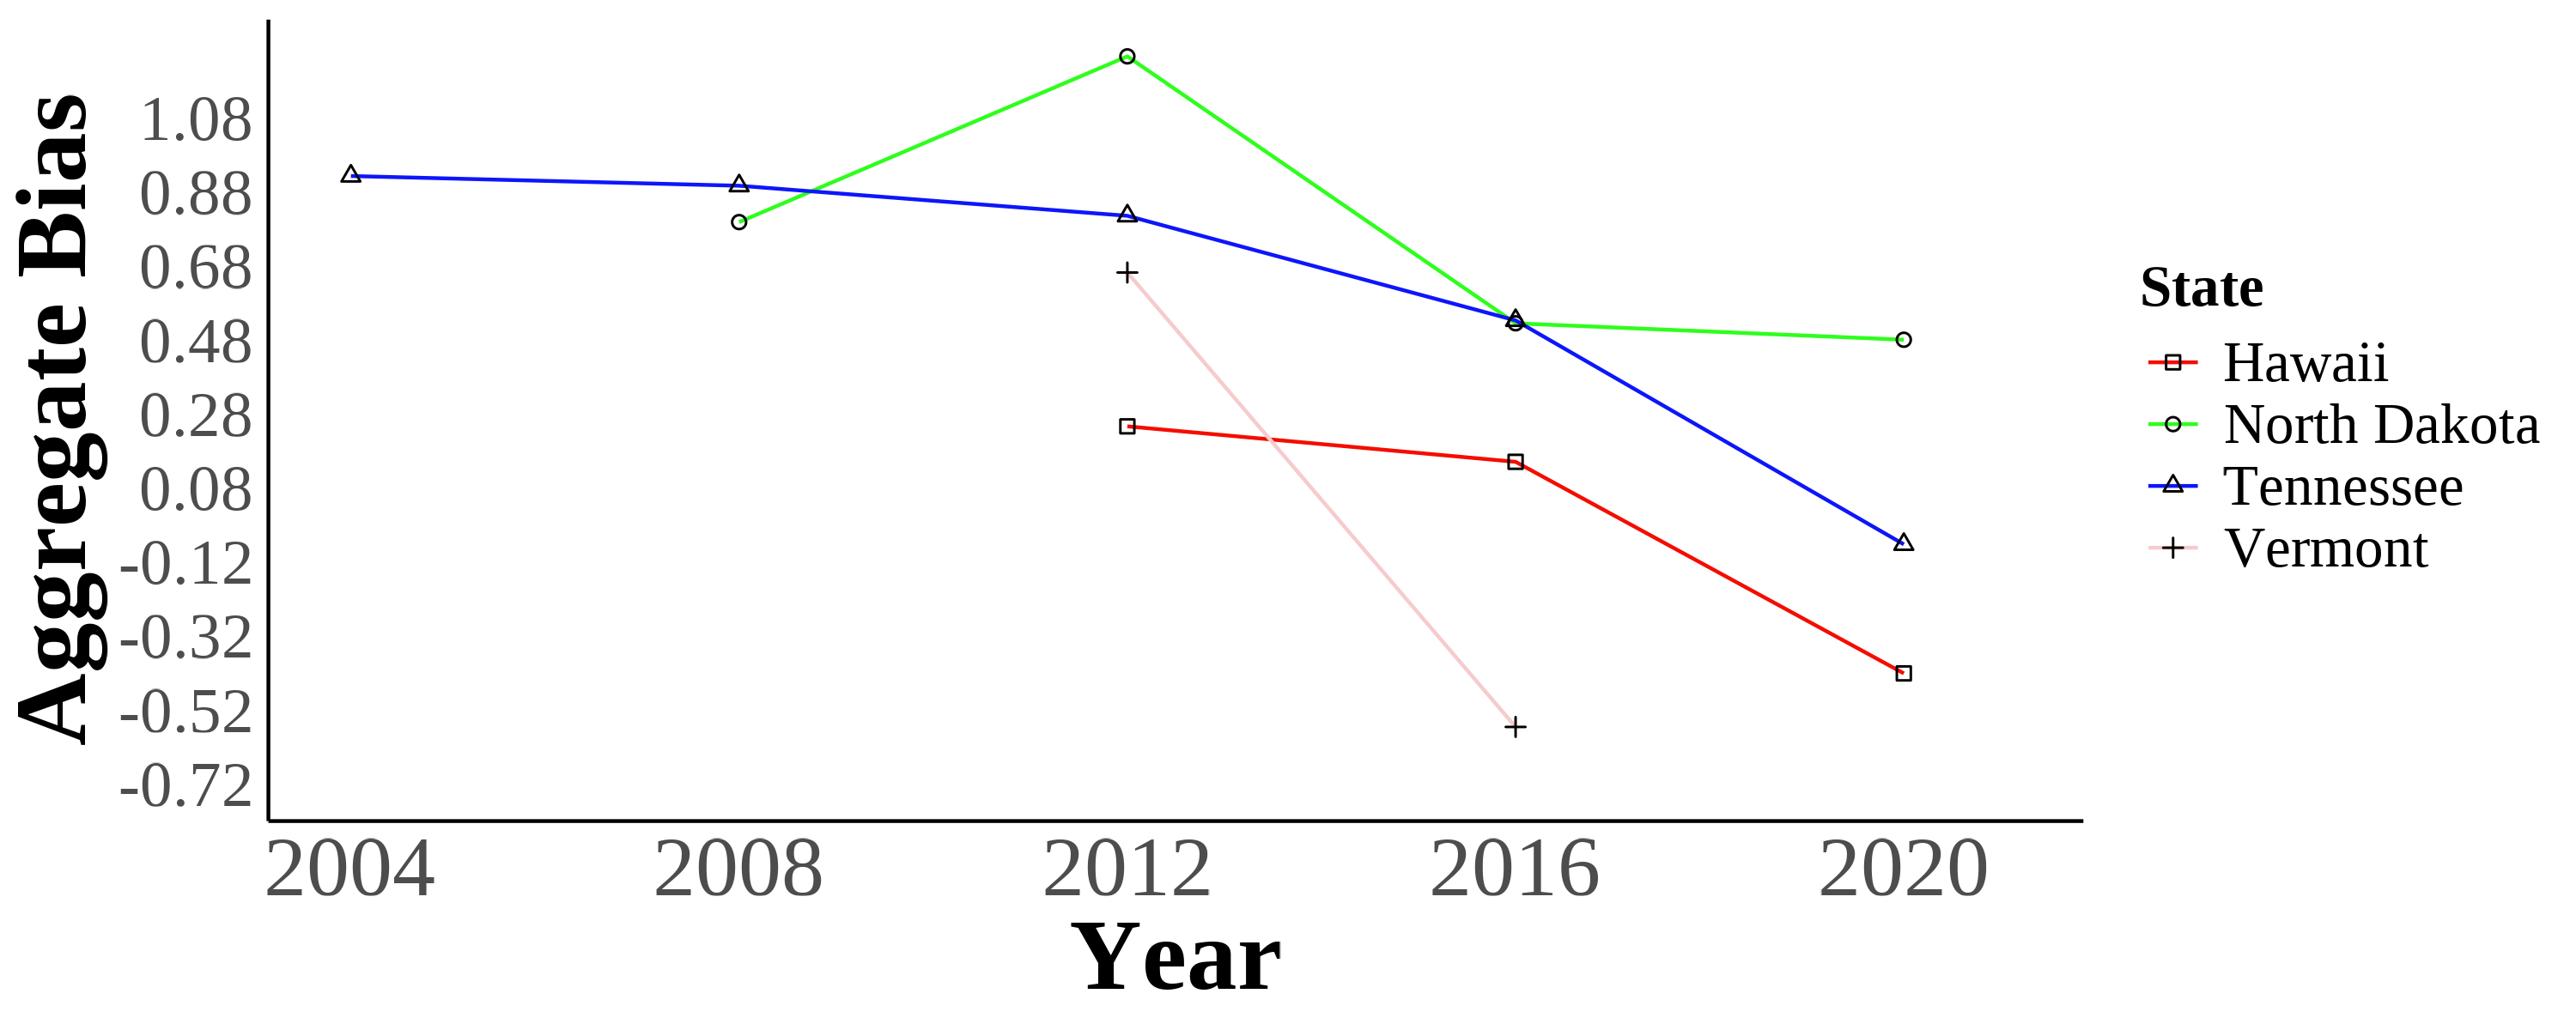
\includegraphics[width=.9\linewidth]{figure/Bias_twostates.png} 
\label{fig:skiniat}
\end{subfigure}
% Second
\begin{subfigure}{.9\textwidth}
\caption{Self-reported Asian Identity Over Time}
\centering
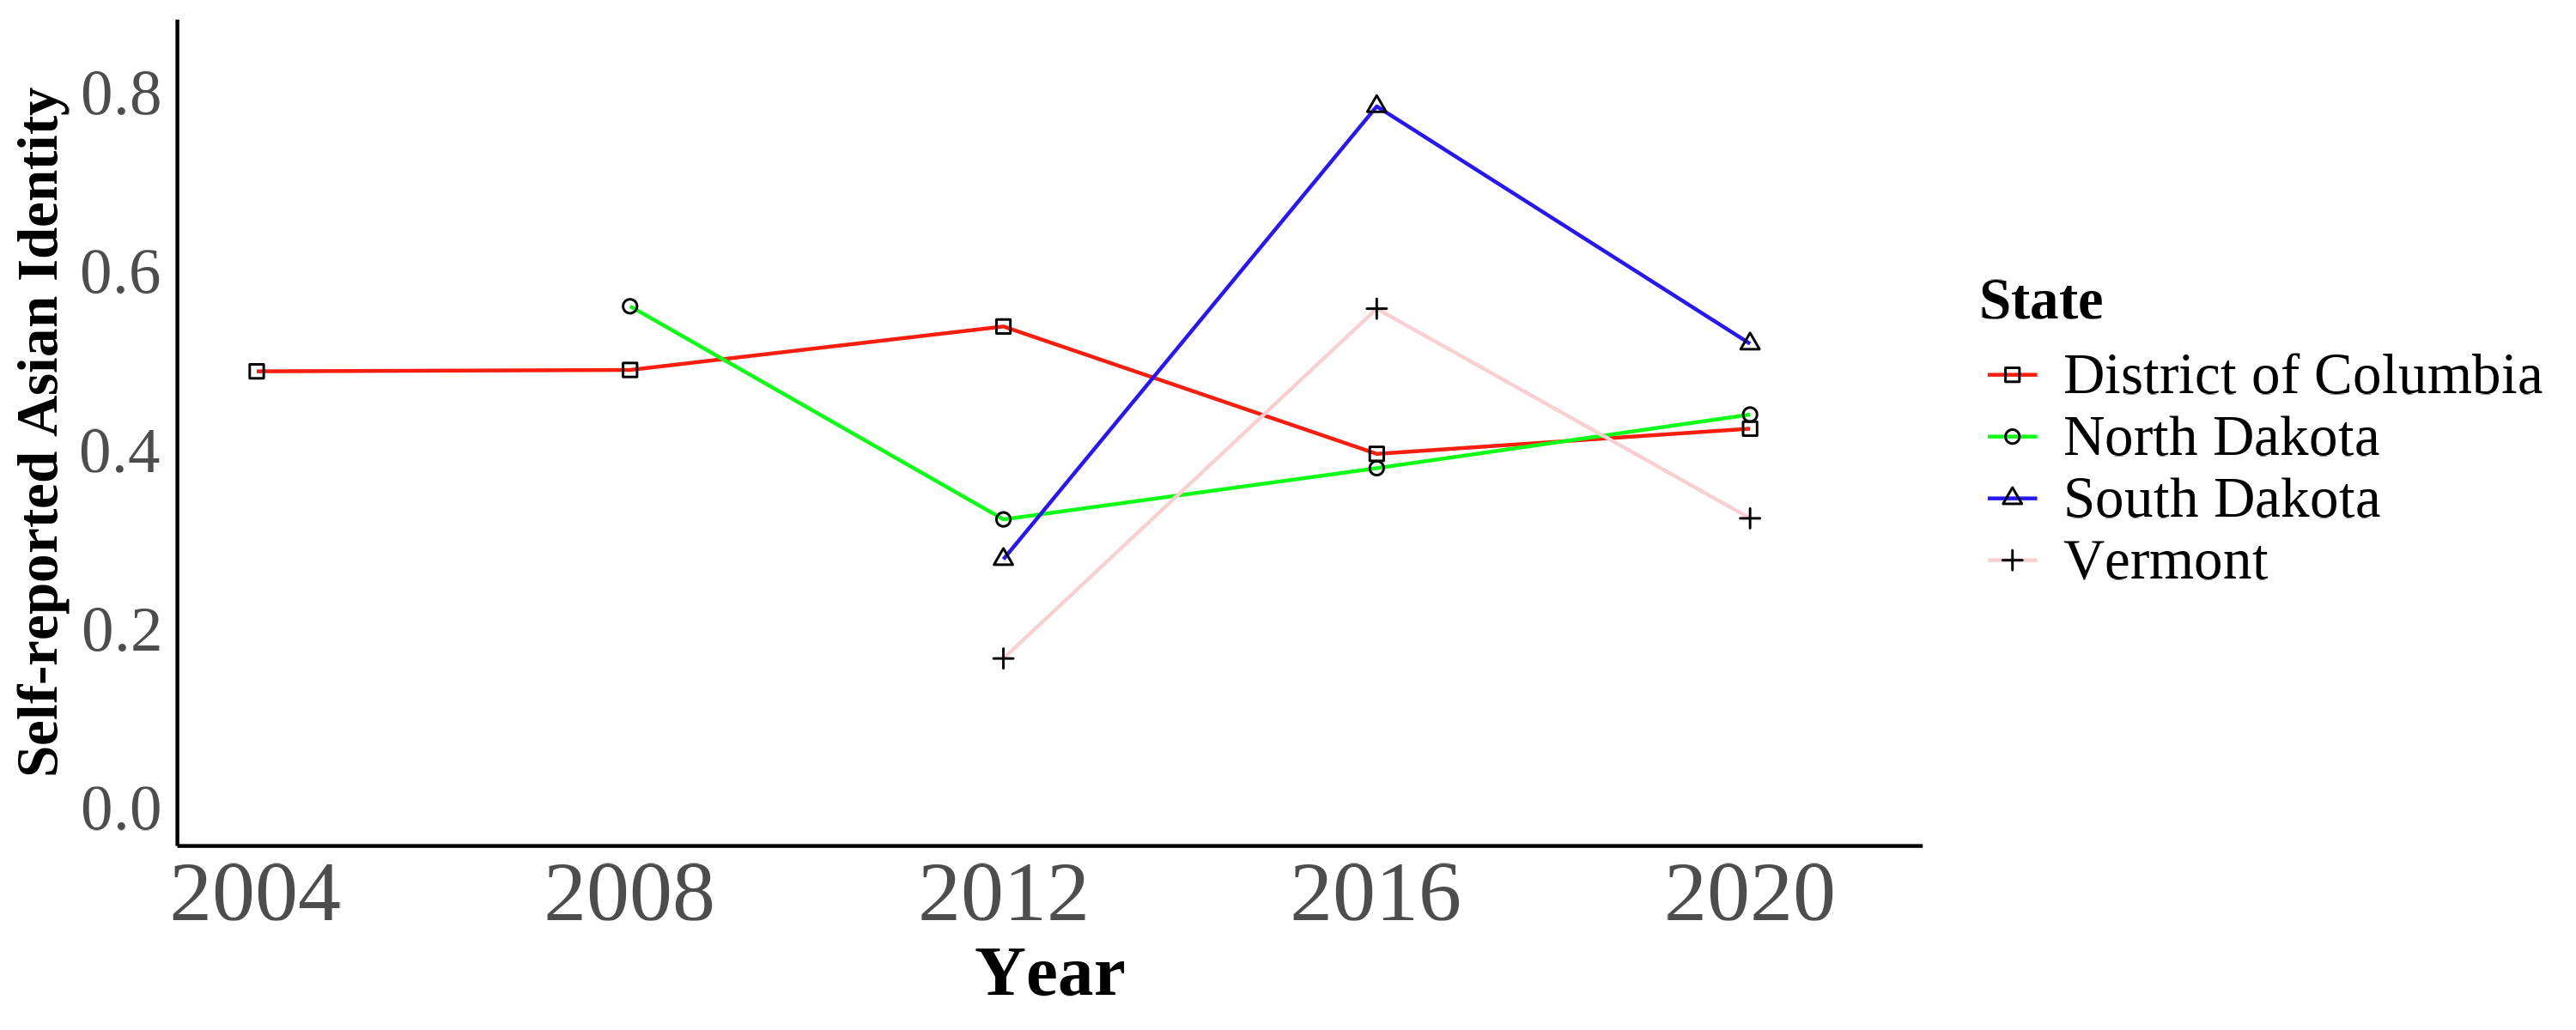
\includegraphics[width=.9\linewidth]{figure/Bias_twostates-asian.png} 
\label{fig:Asian-twostates}
\end{subfigure}
\caption*{\footnotesize{These two panels show the trends in implicit bias (panel a) and self-reported Asian identity among Asian immigrants (panel b) of the least and most biased places in the data. The District of Colombia is the least biased geographical area, and North Dakota is the most biased. The bias units are in standard deviations. Self-reported Asian identity is among first, second, and third-generation Asian immigrants aged 17 and younger still living in intact families.\\
Bias data is from the 2004-2021 Harvard's Project Implicit Association Test scores. Identity data is from the 2004-2021 Current Population Survey (CPS).}}
\end{figure}
\end{center}


\newpage
\pagebreak

\begin{center}
\begin{figure}[H]
\caption{Maps of State-level Implicit Association Test Bias Over Time Measure with Census Division Regional Boundaries}
\label{fig:skiniat-maps}
% first
\begin{subfigure}{.45\textwidth}
\caption{State-level Bias in 2004}
\centering
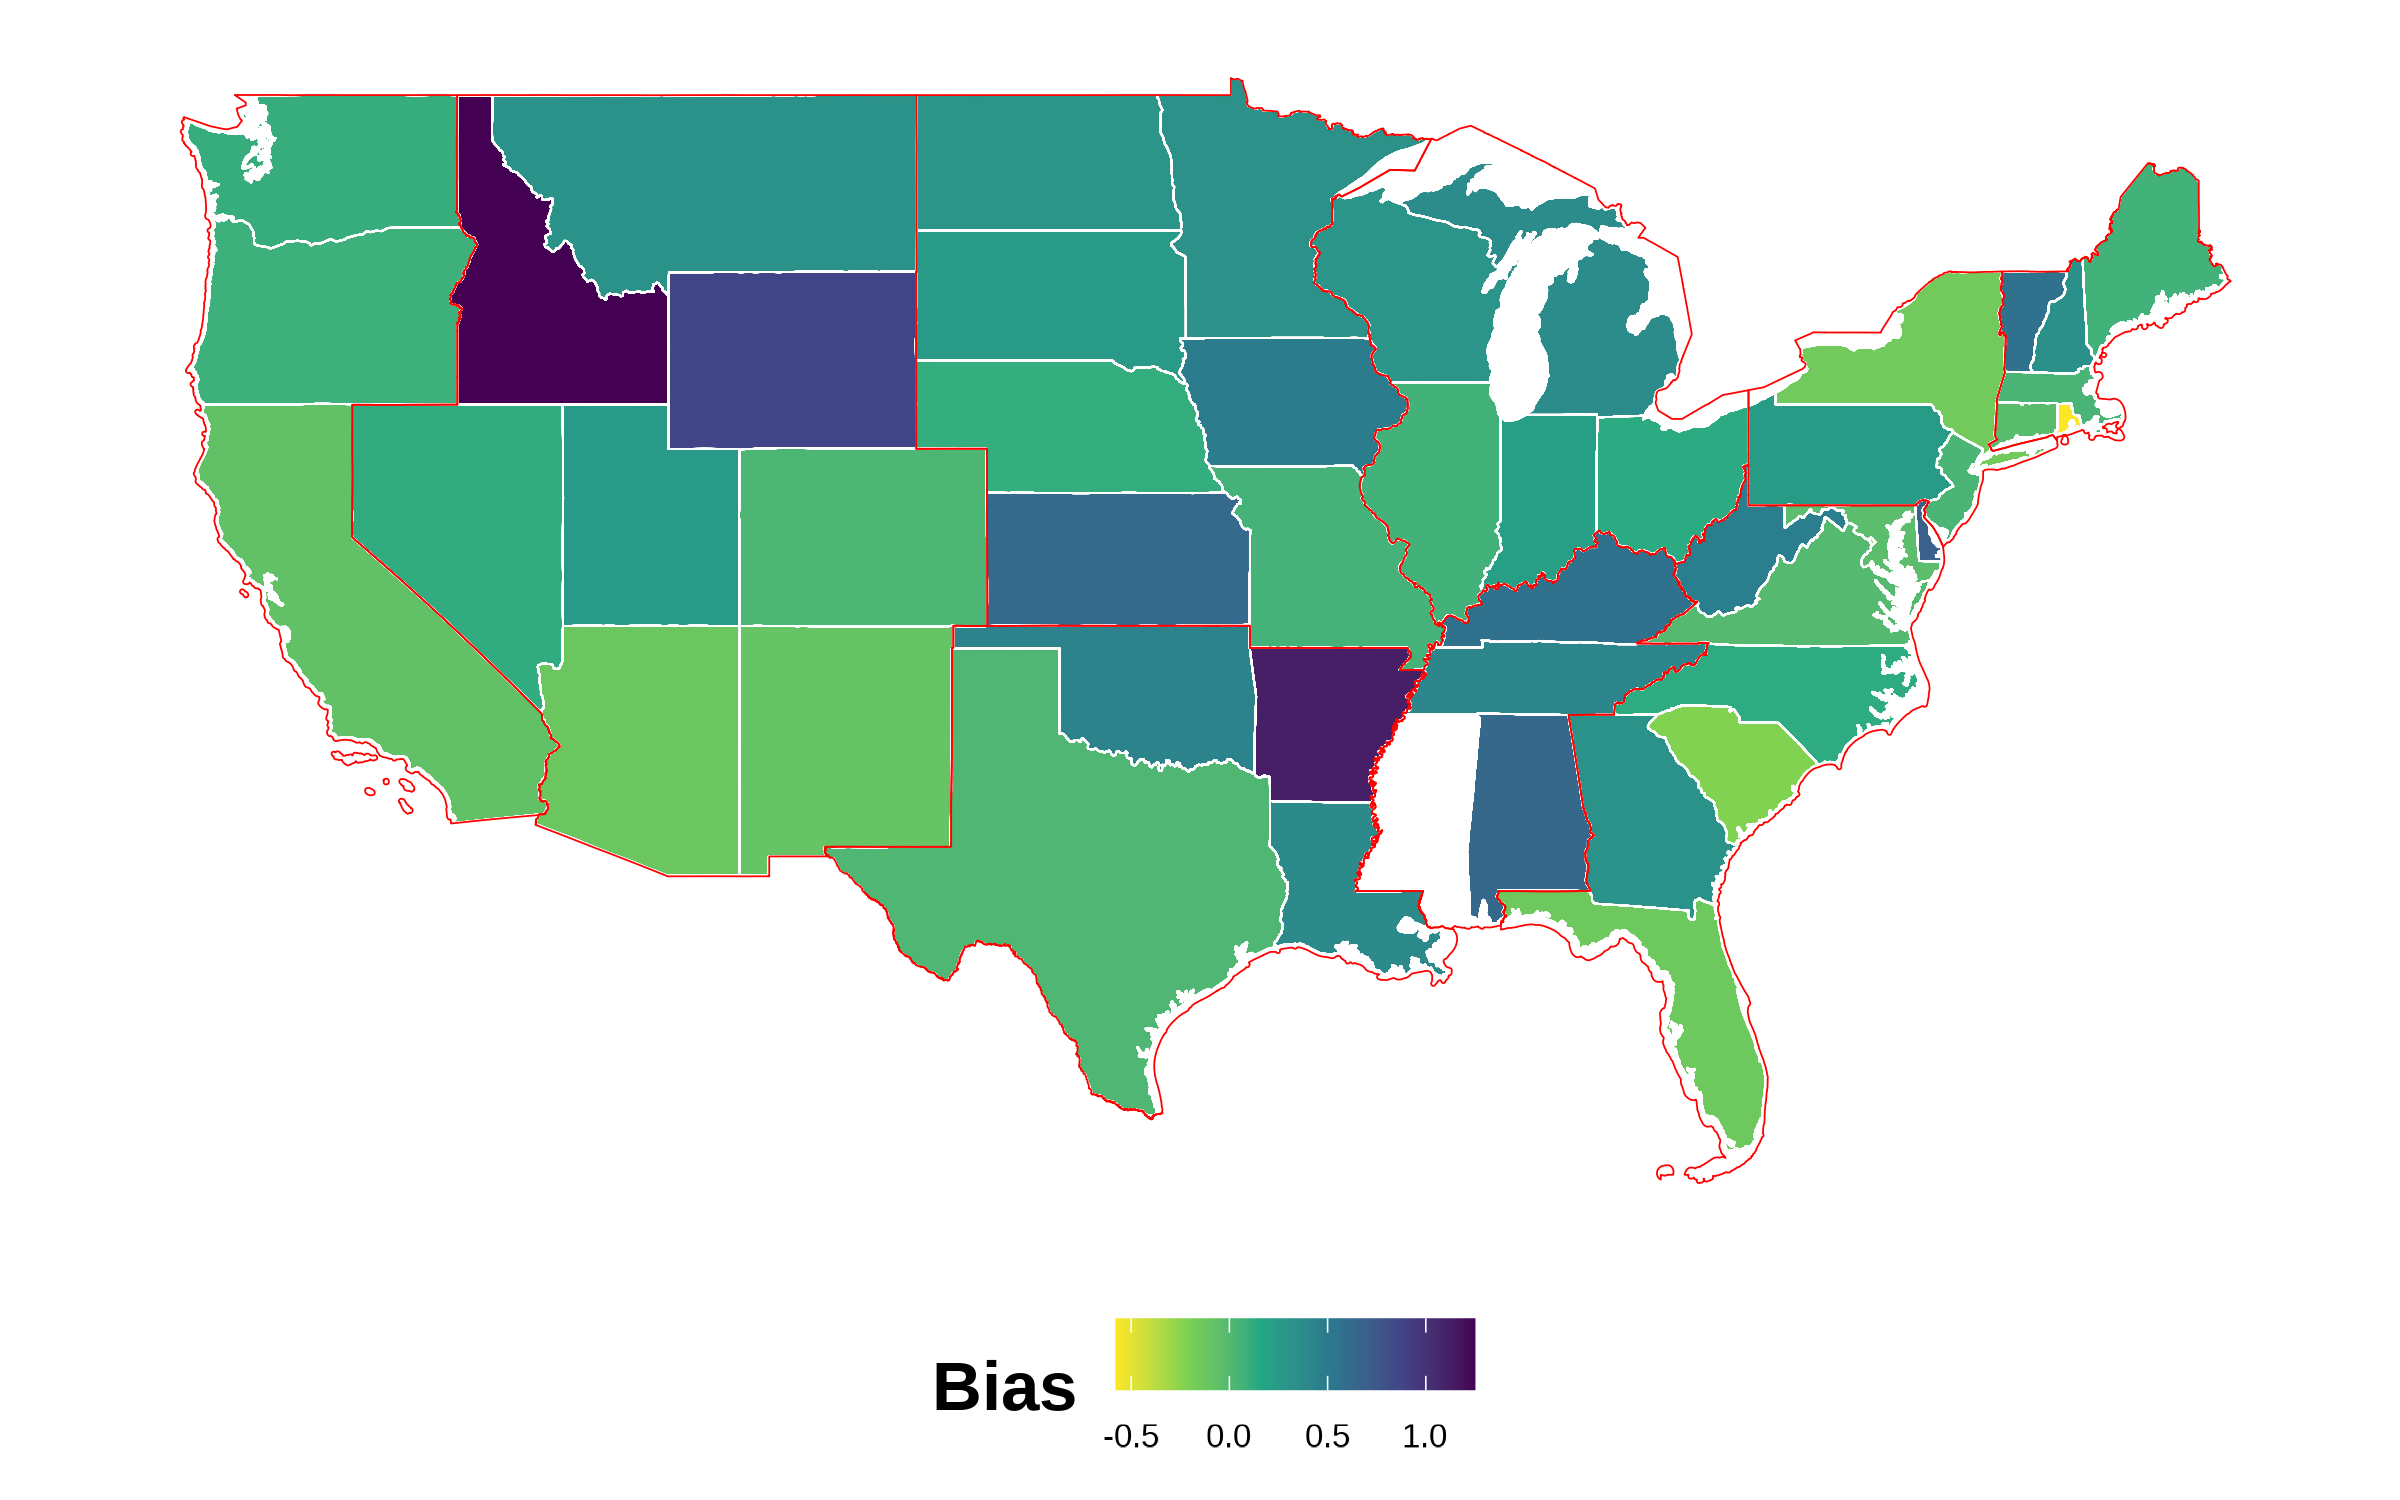
\includegraphics[width=0.9\linewidth]{figure/2004skinmap.png} 
\label{fig:skiniat-map-2004}
\end{subfigure}
\hfill%
% Second
\begin{subfigure}{.45\textwidth}
\caption{State-level Bias in 2008}
\centering
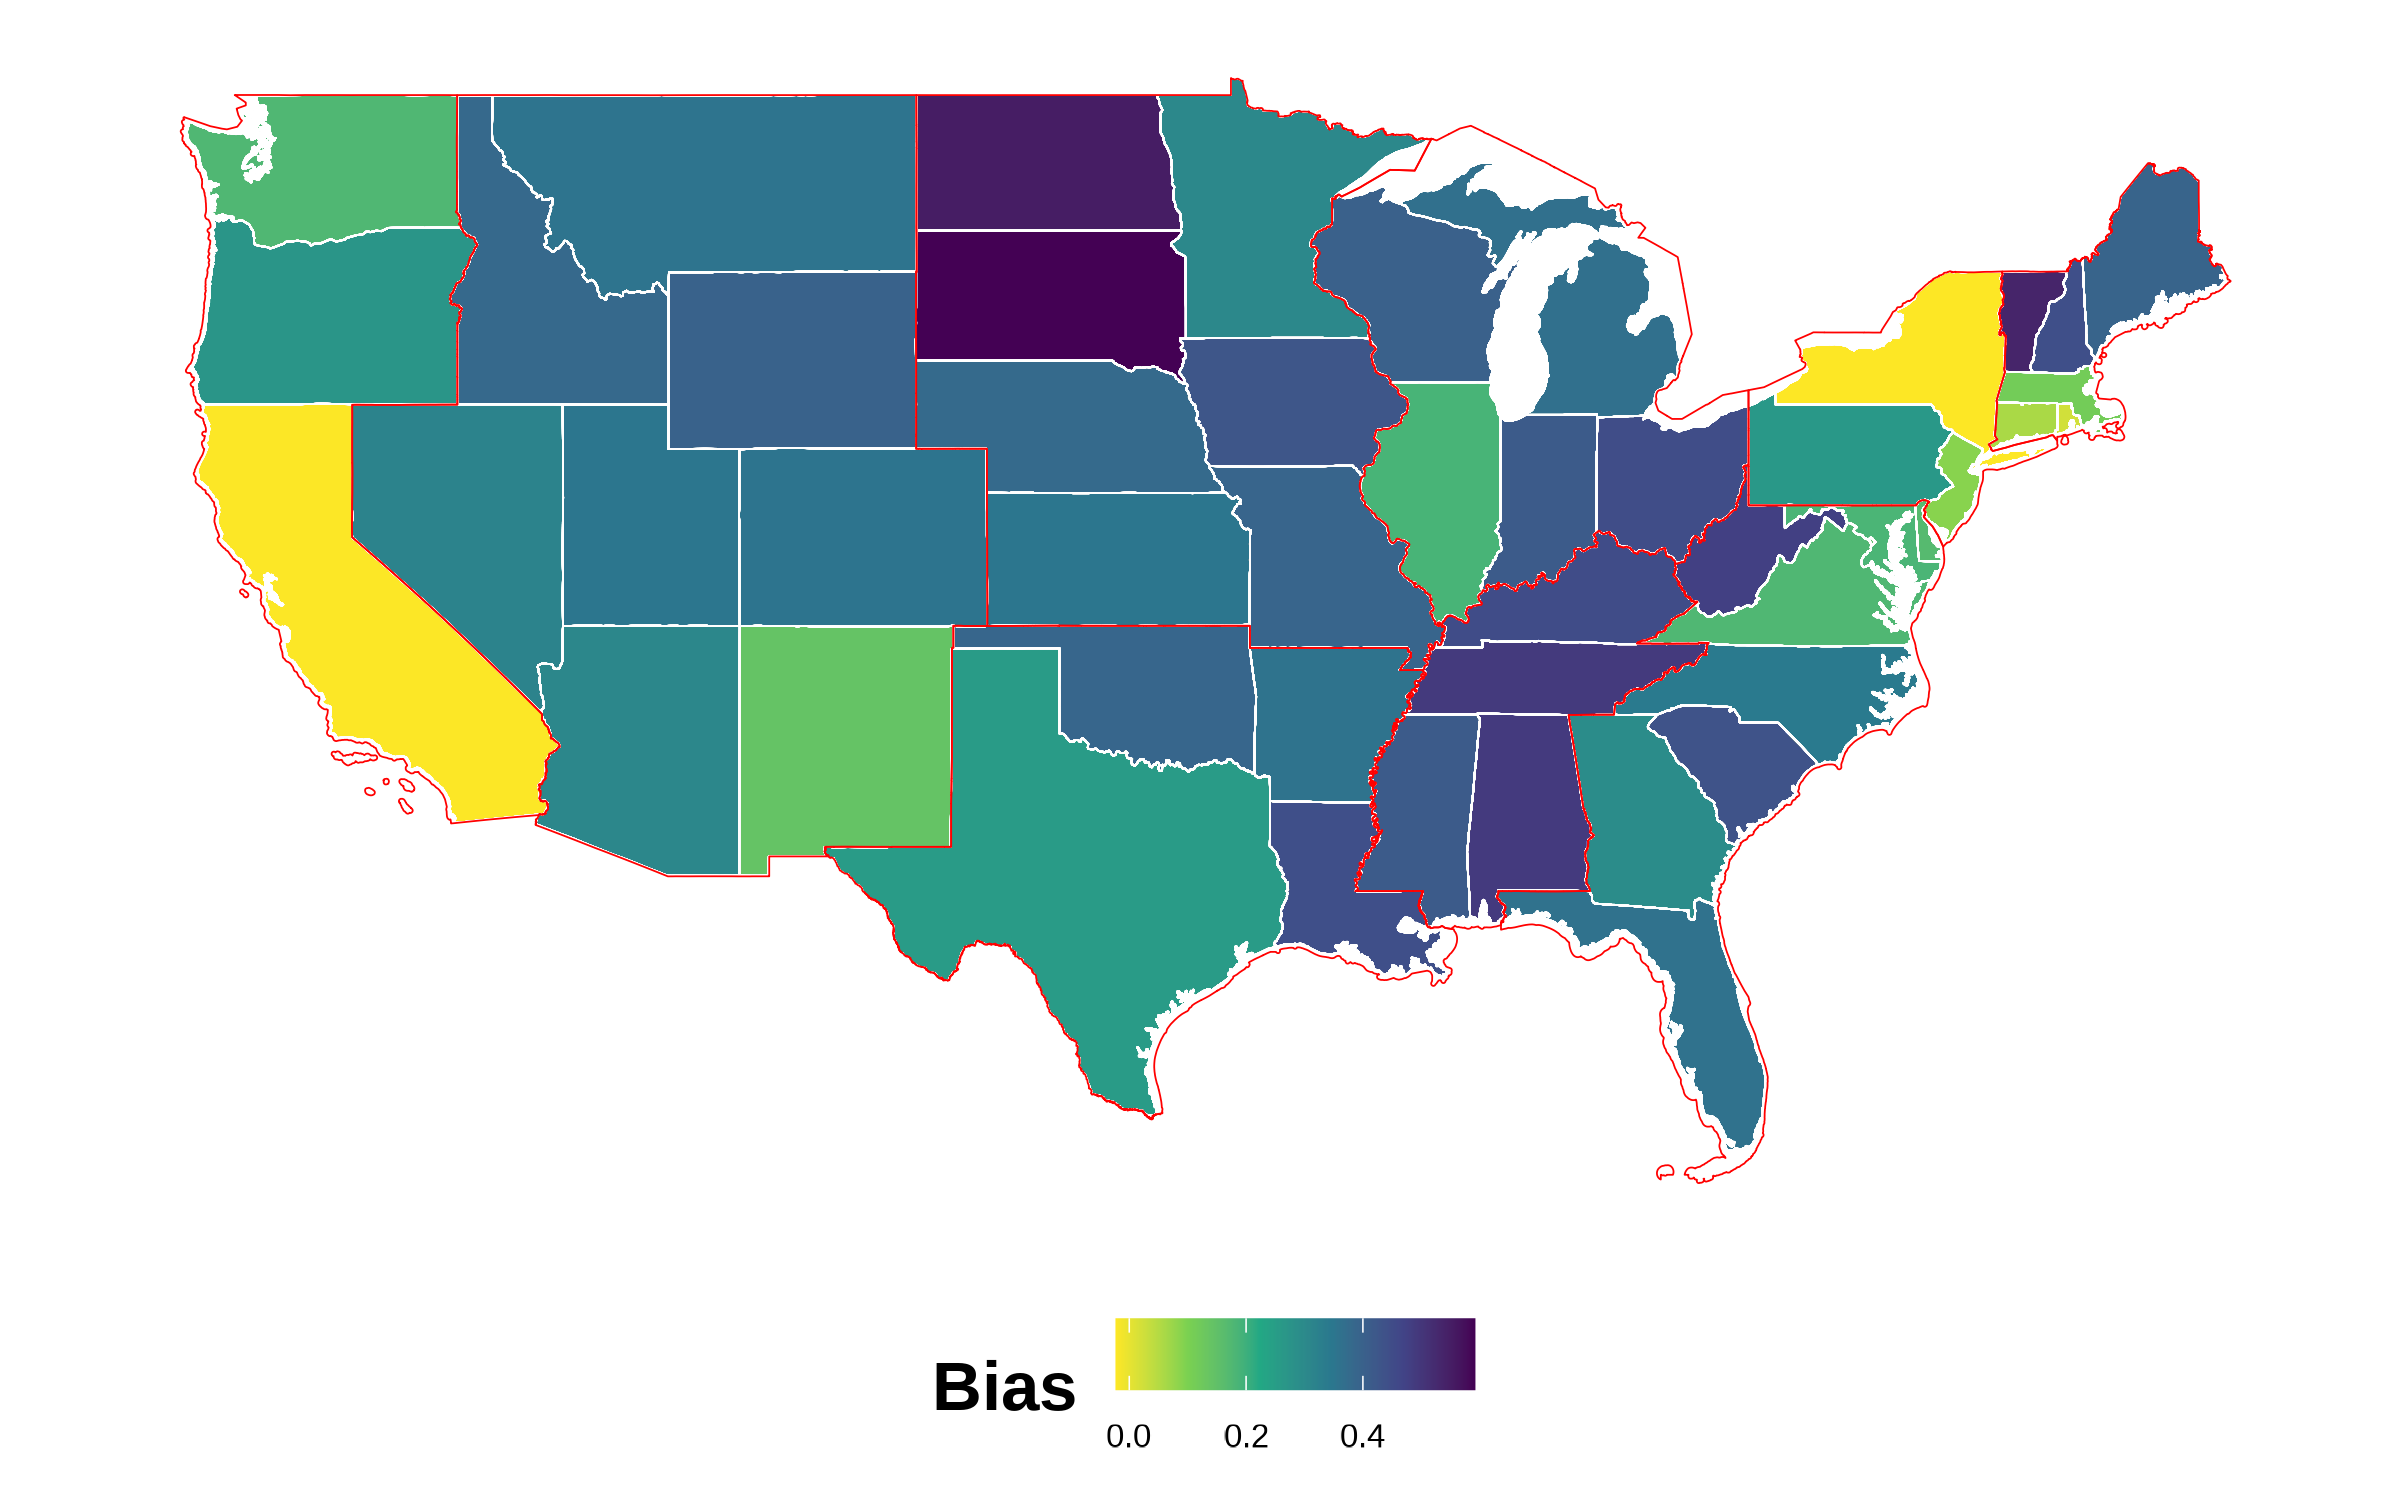
\includegraphics[width=0.9\linewidth]{figure/2008skinmap.png} 
\label{fig:skiniat-map-2006}
\end{subfigure}
\hfill%
% third
\begin{subfigure}{.45\textwidth}
\caption{State-level Bias in 2012}
\centering
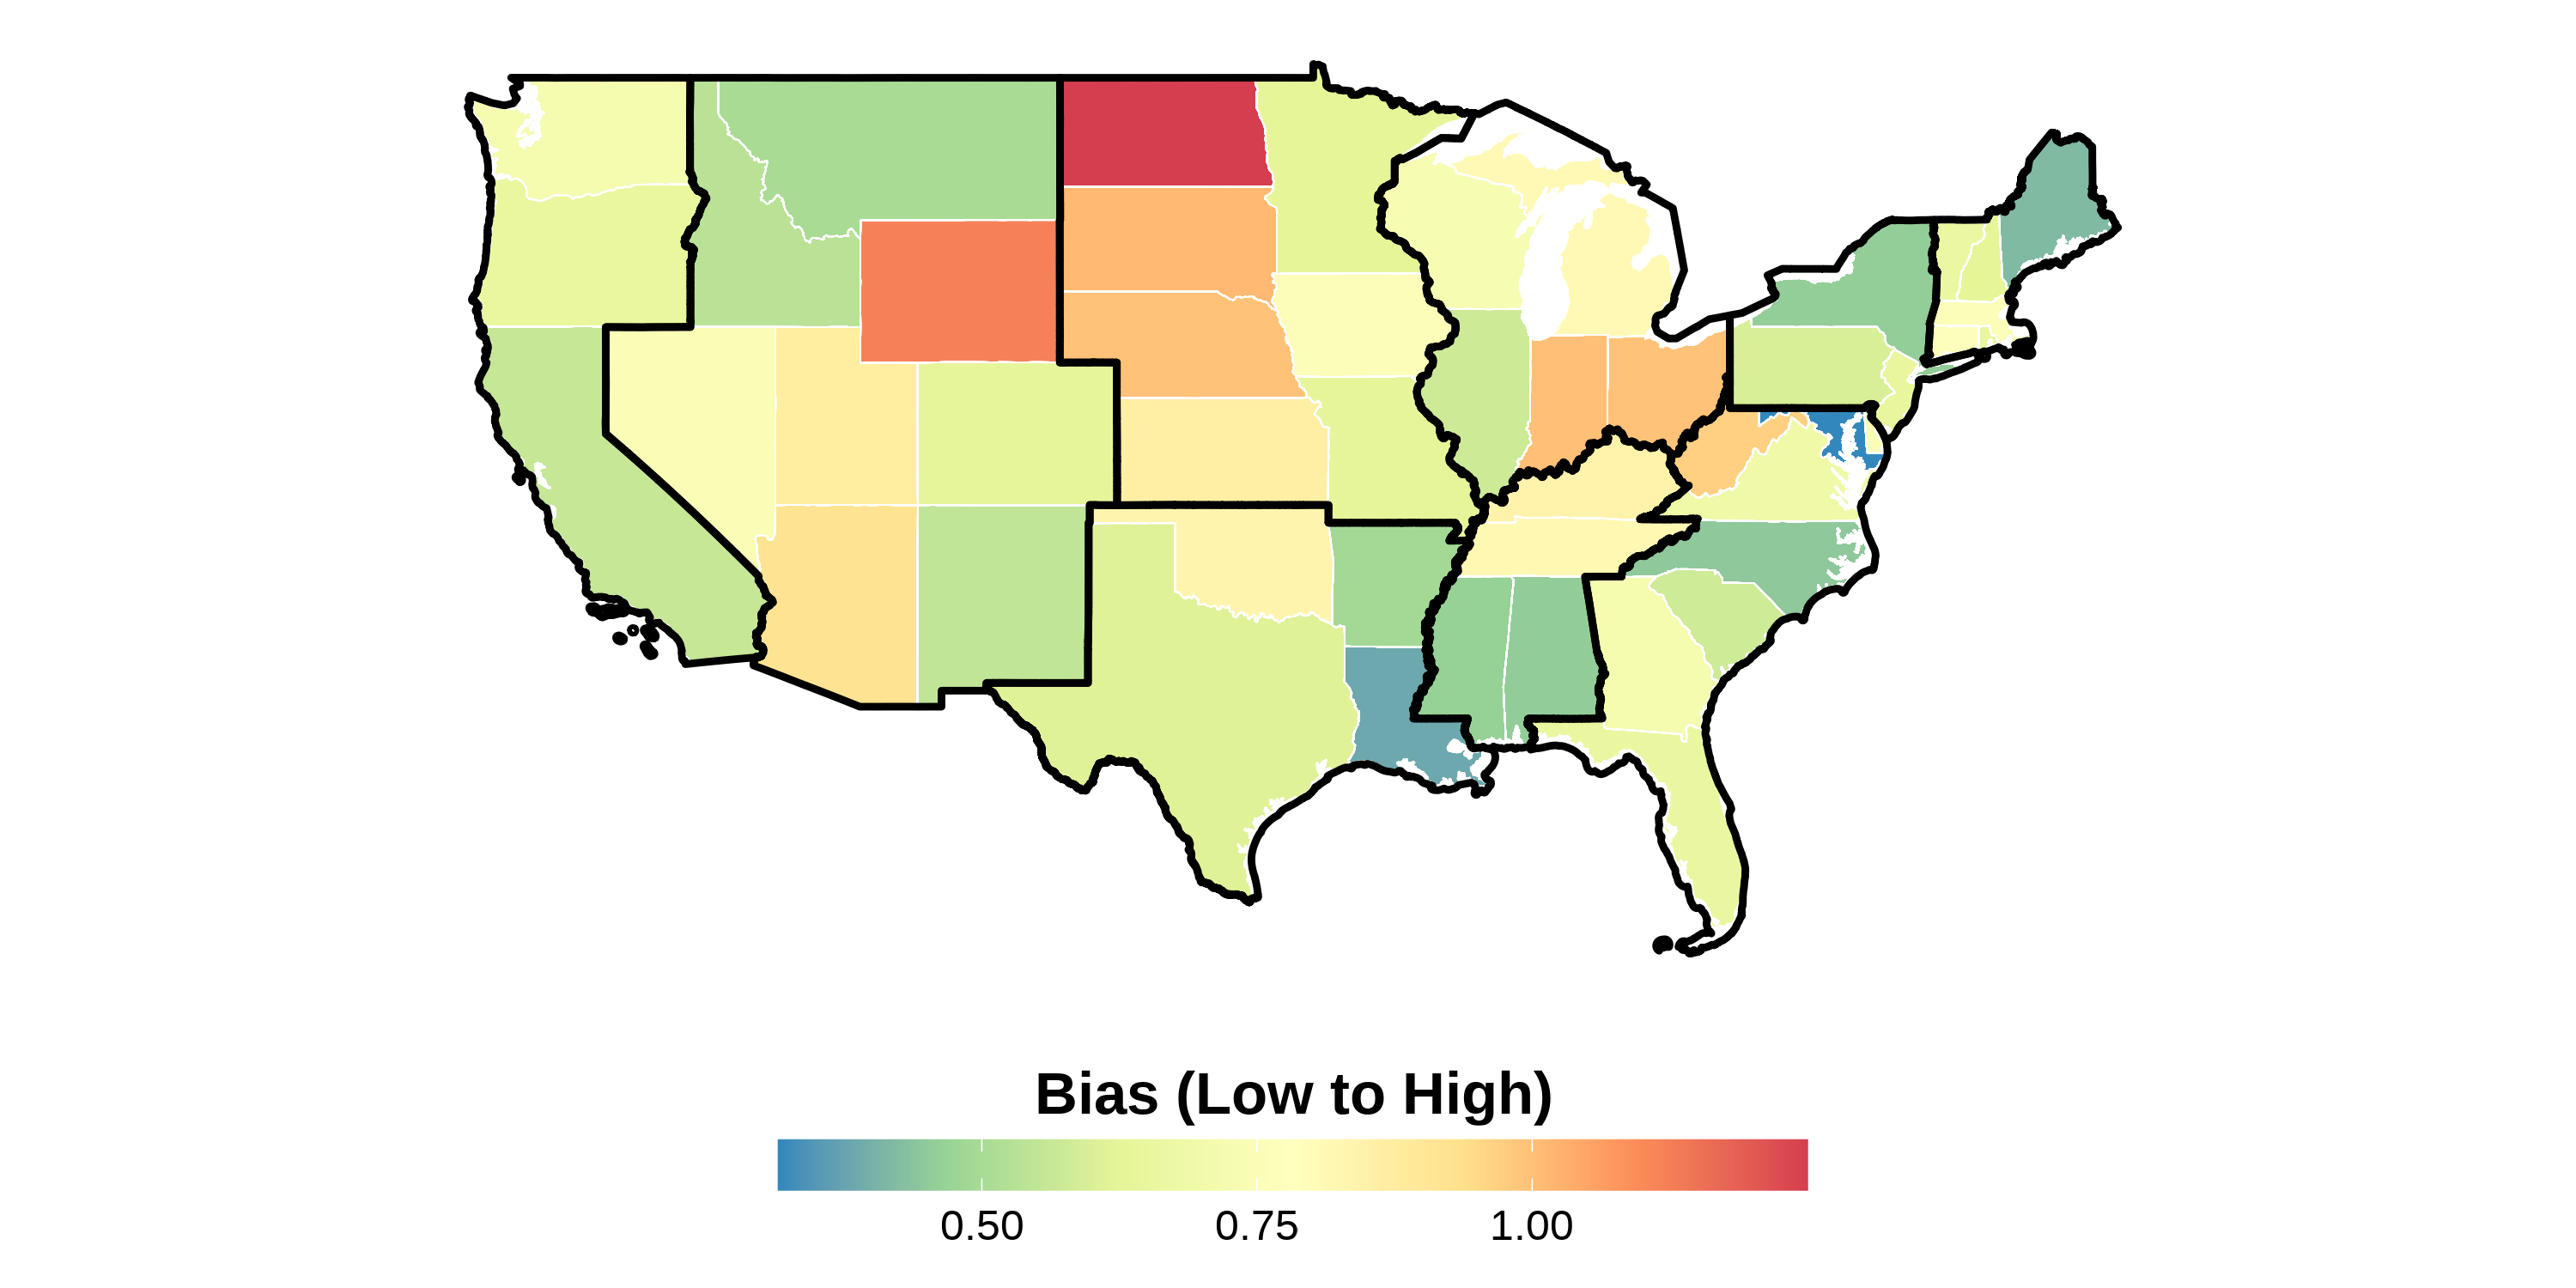
\includegraphics[width=0.9\linewidth]{figure/2012skinmap.png} 
\label{fig:skiniat-map-2008}
\end{subfigure}
\hfill%
% fourth
\begin{subfigure}{.45\textwidth}
\caption{State-level Bias in 2016}
\centering
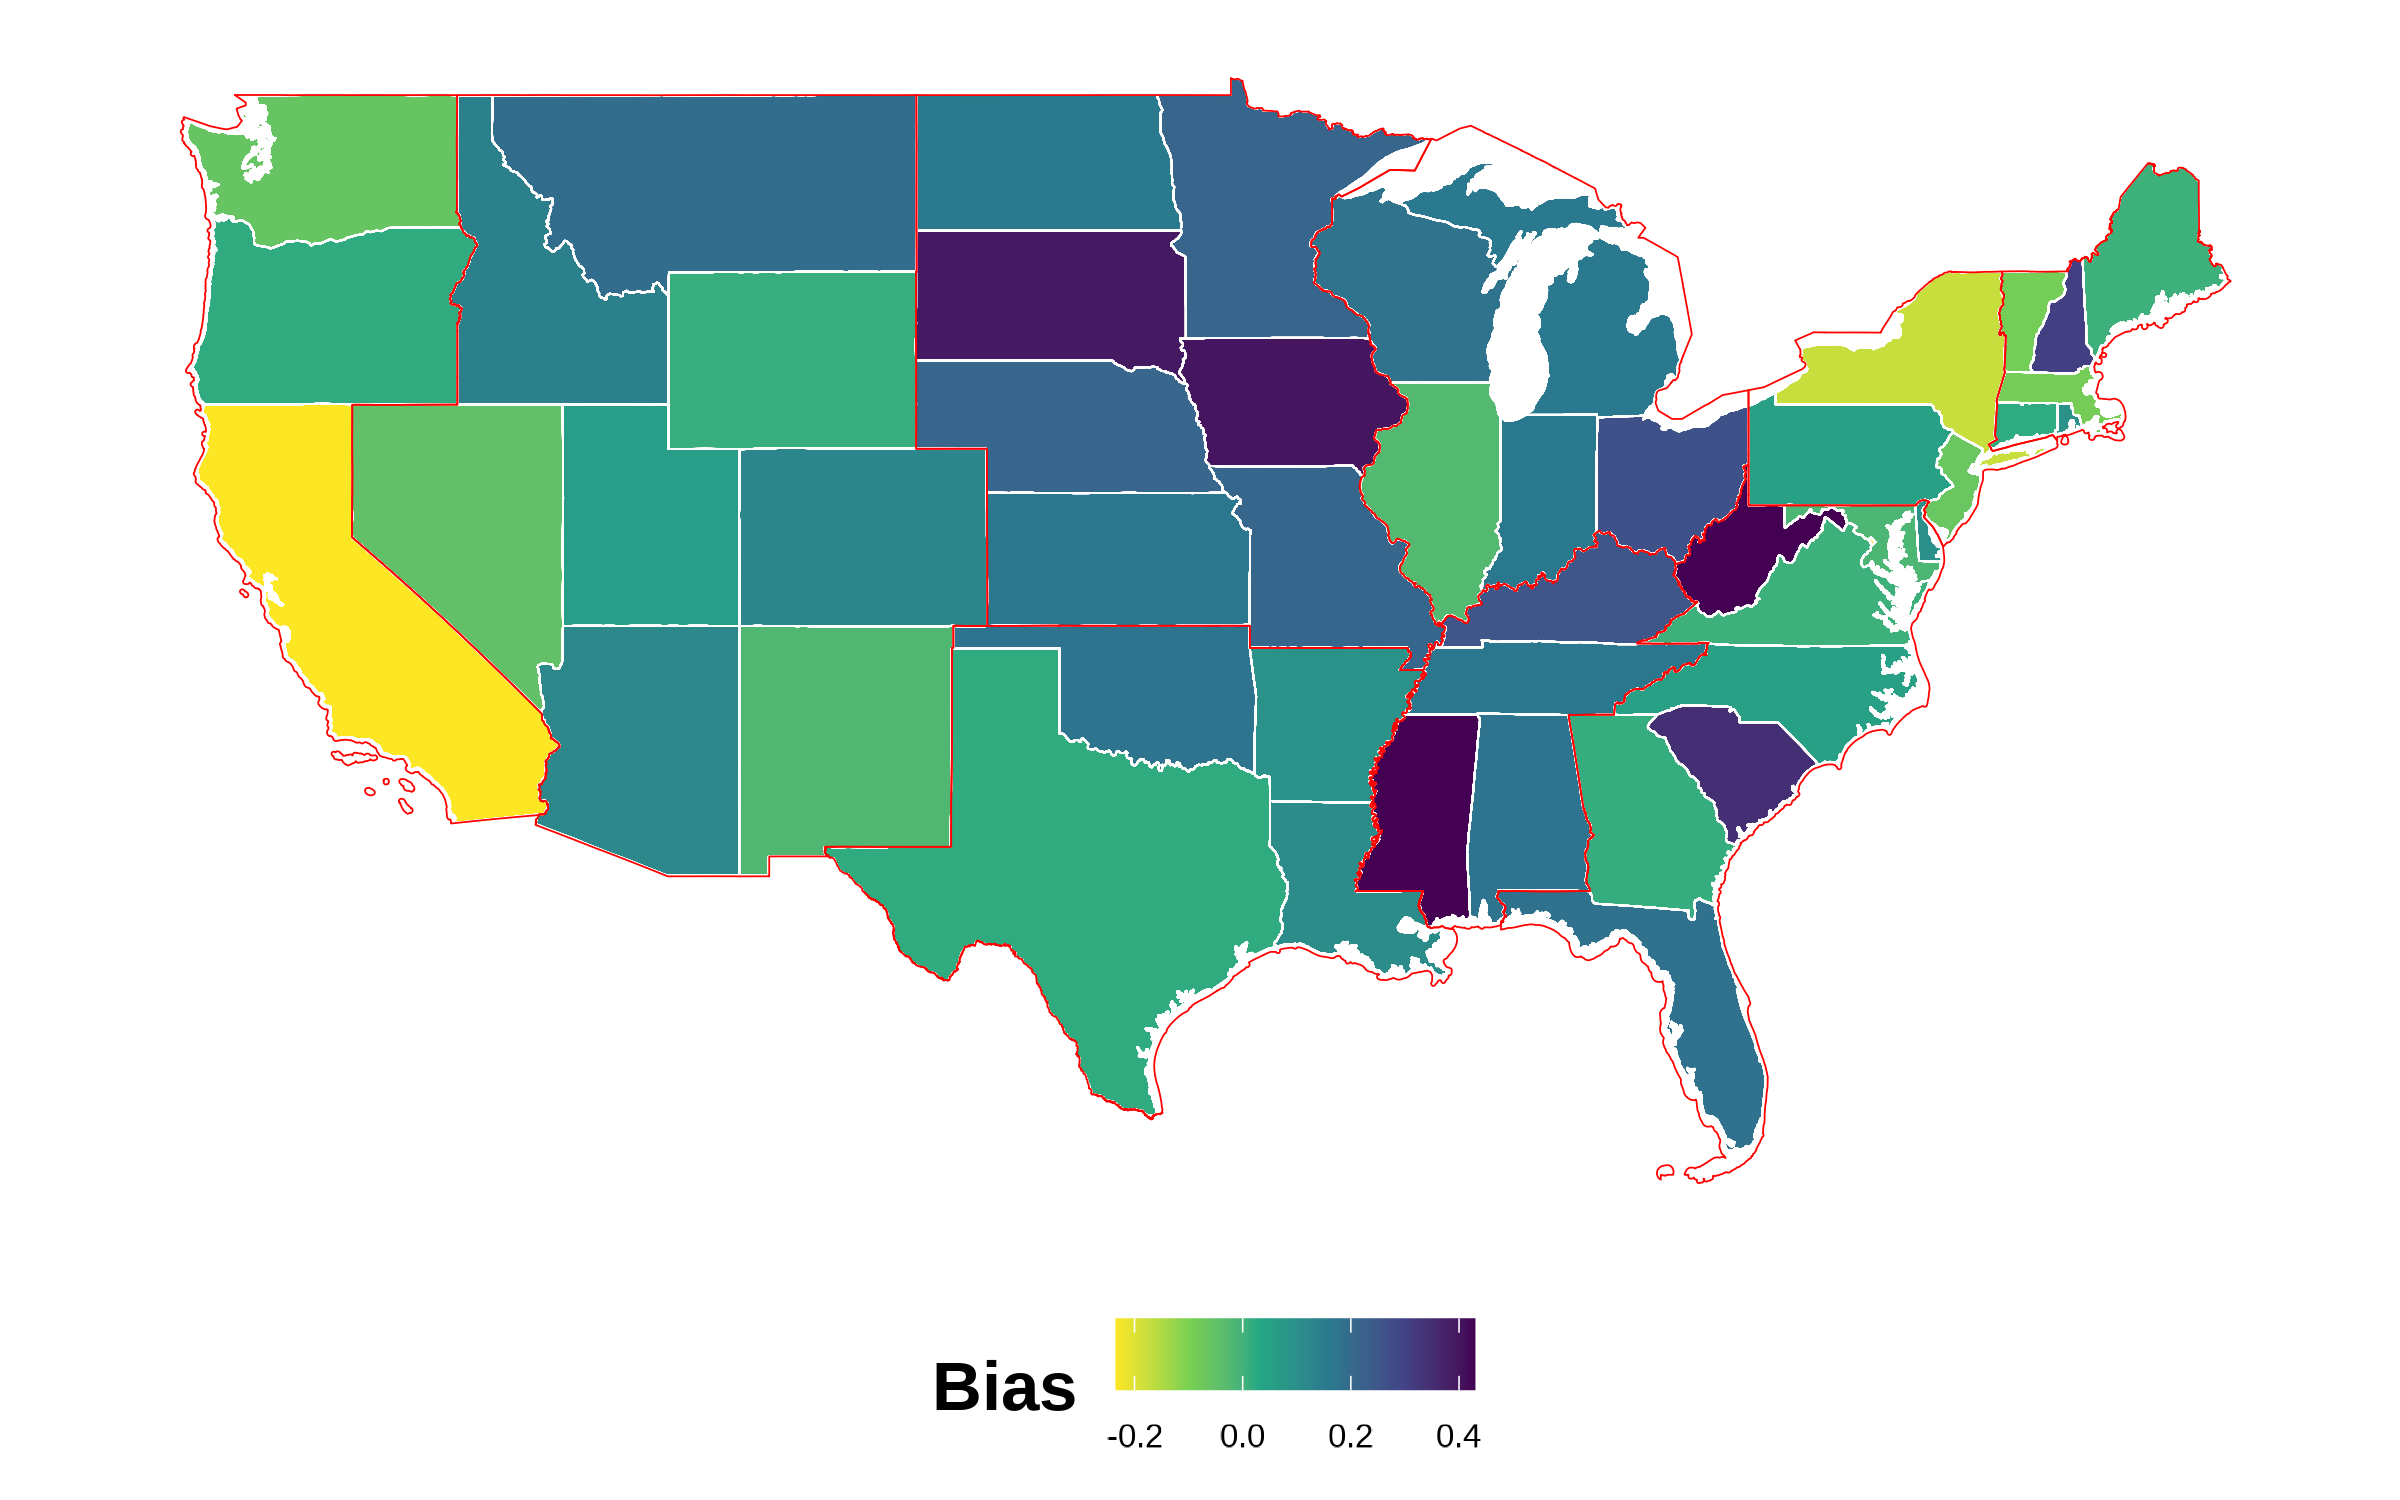
\includegraphics[width=0.9\linewidth]{figure/2016skinmap.png} 
\label{fig:skiniat-map-2010}
\end{subfigure}

\caption*{\footnotesize{In this figure, I show the state-level implicit bias in different years in the sample. Each panel presents state-level bias during a certain year. The boundaries in red represent the different Census divisions in the United States. Notice how there is a variation across states with-in a region.}}
\end{figure}
\end{center}

\pagebreak
\newpage

\begin{center}
\begin{figure}[!htb]
\centering
\caption{Relationship Between Self-Reported Asian Identity and Bias: By Generation}
\label{plot01-regression-gen}
%First graph
\begin{subfigure}{.48\textwidth}
\caption{All Generations}
\centering
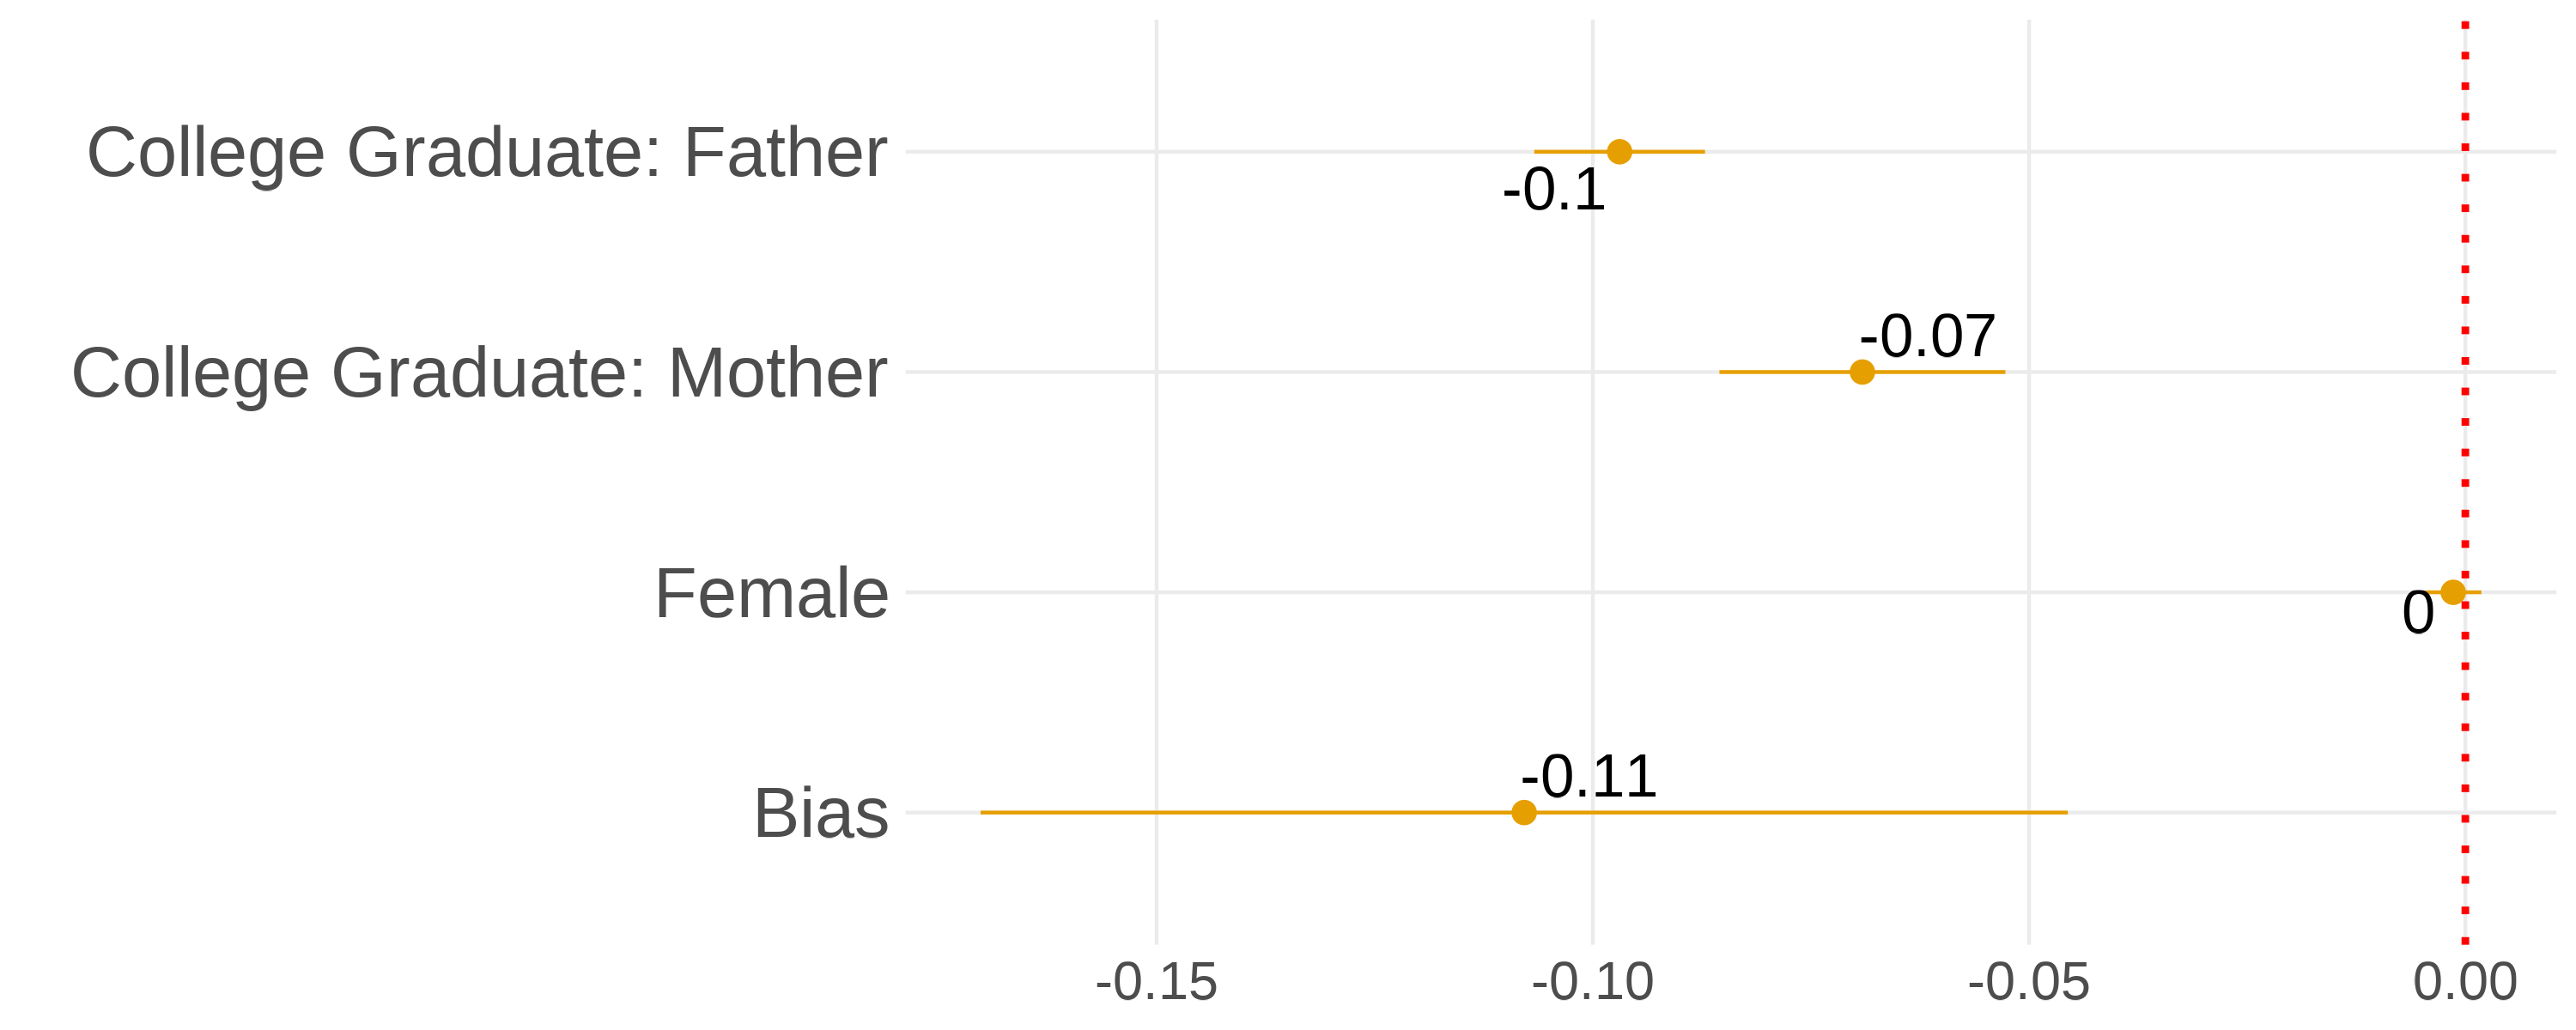
\includegraphics[width=.9\linewidth]{figure/skin-iat-regression-all-gens.png}
\end{subfigure}
\centering
%Second graph
\begin{subfigure}{.48\textwidth}
\caption{First-Generation}
\centering
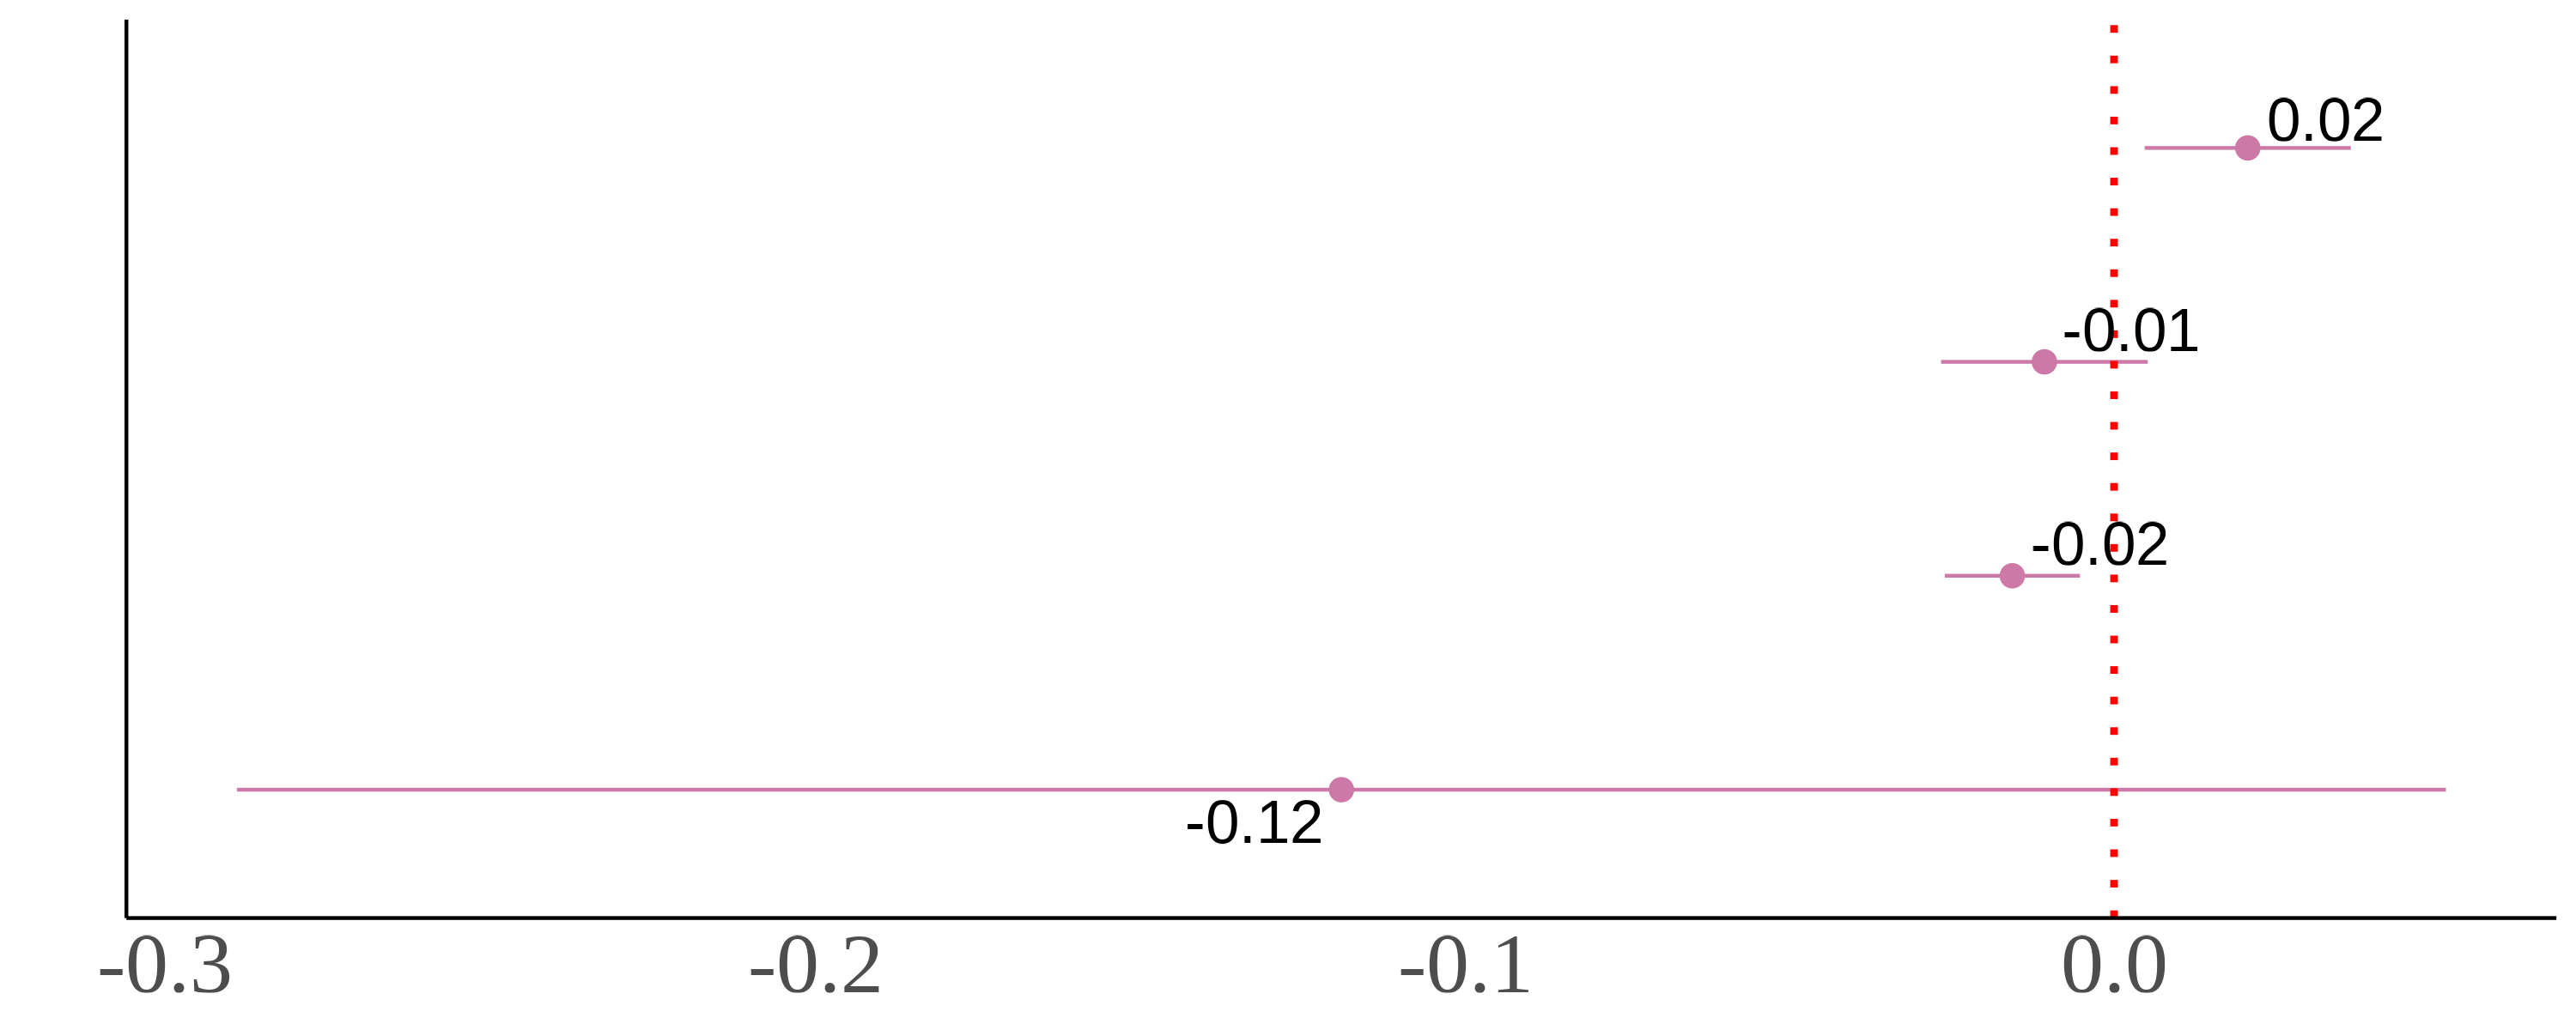
\includegraphics[width=.9\linewidth]{figure/skin-iat-regression-first-gen.png}
\end{subfigure}
%Third Graph
\begin{subfigure}{.48\textwidth}
\caption{Second-Generation}
\centering
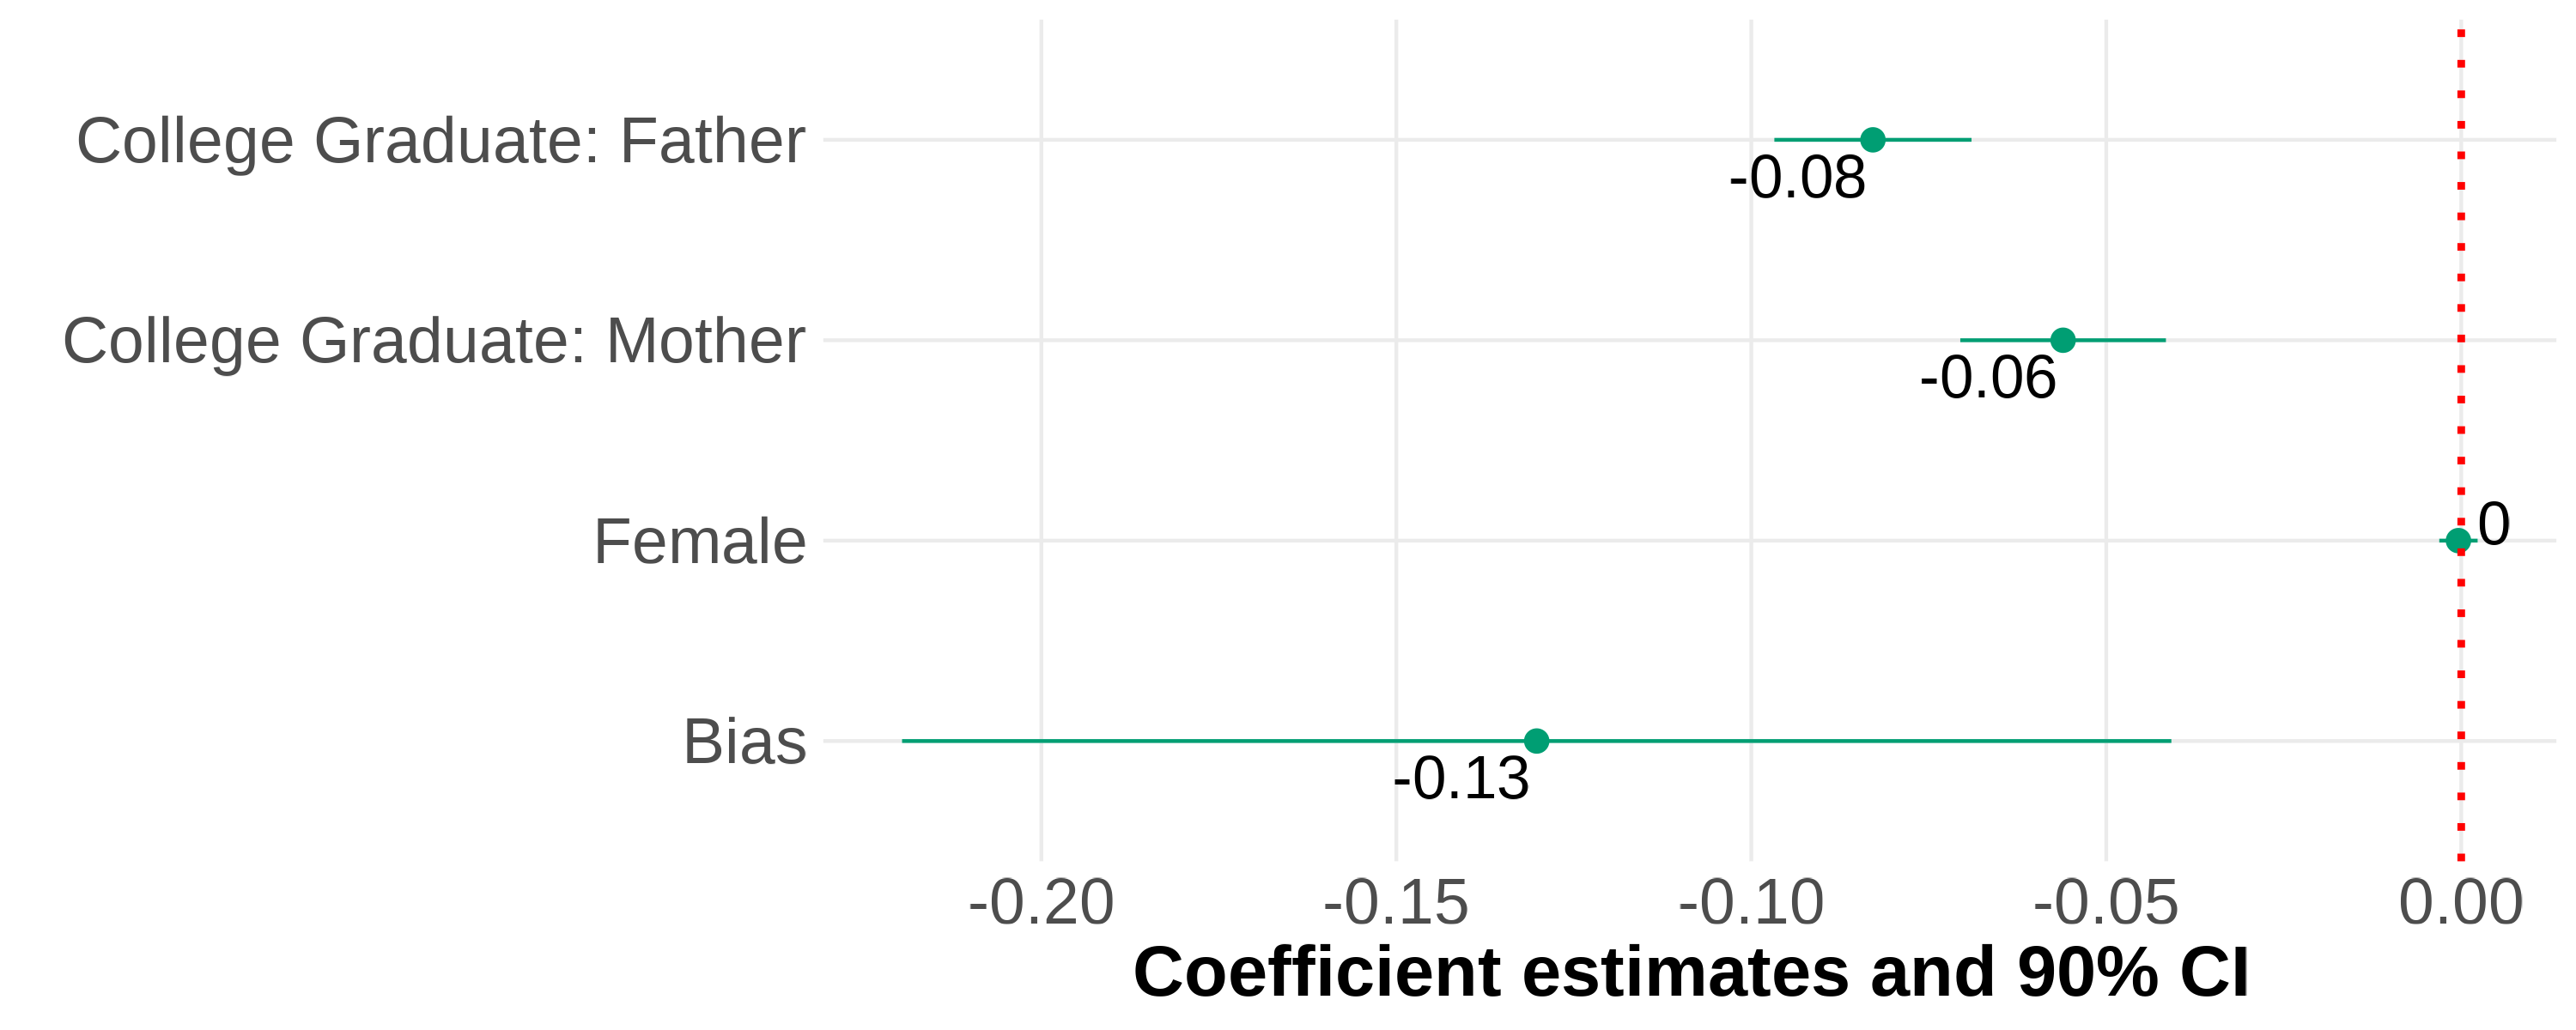
\includegraphics[width=.9\linewidth]{figure/skin-iat-regression-second-gen.png}
\end{subfigure}
%Fourth Graph
\begin{subfigure}{.48\textwidth}
\caption{Third-Generation}
\centering
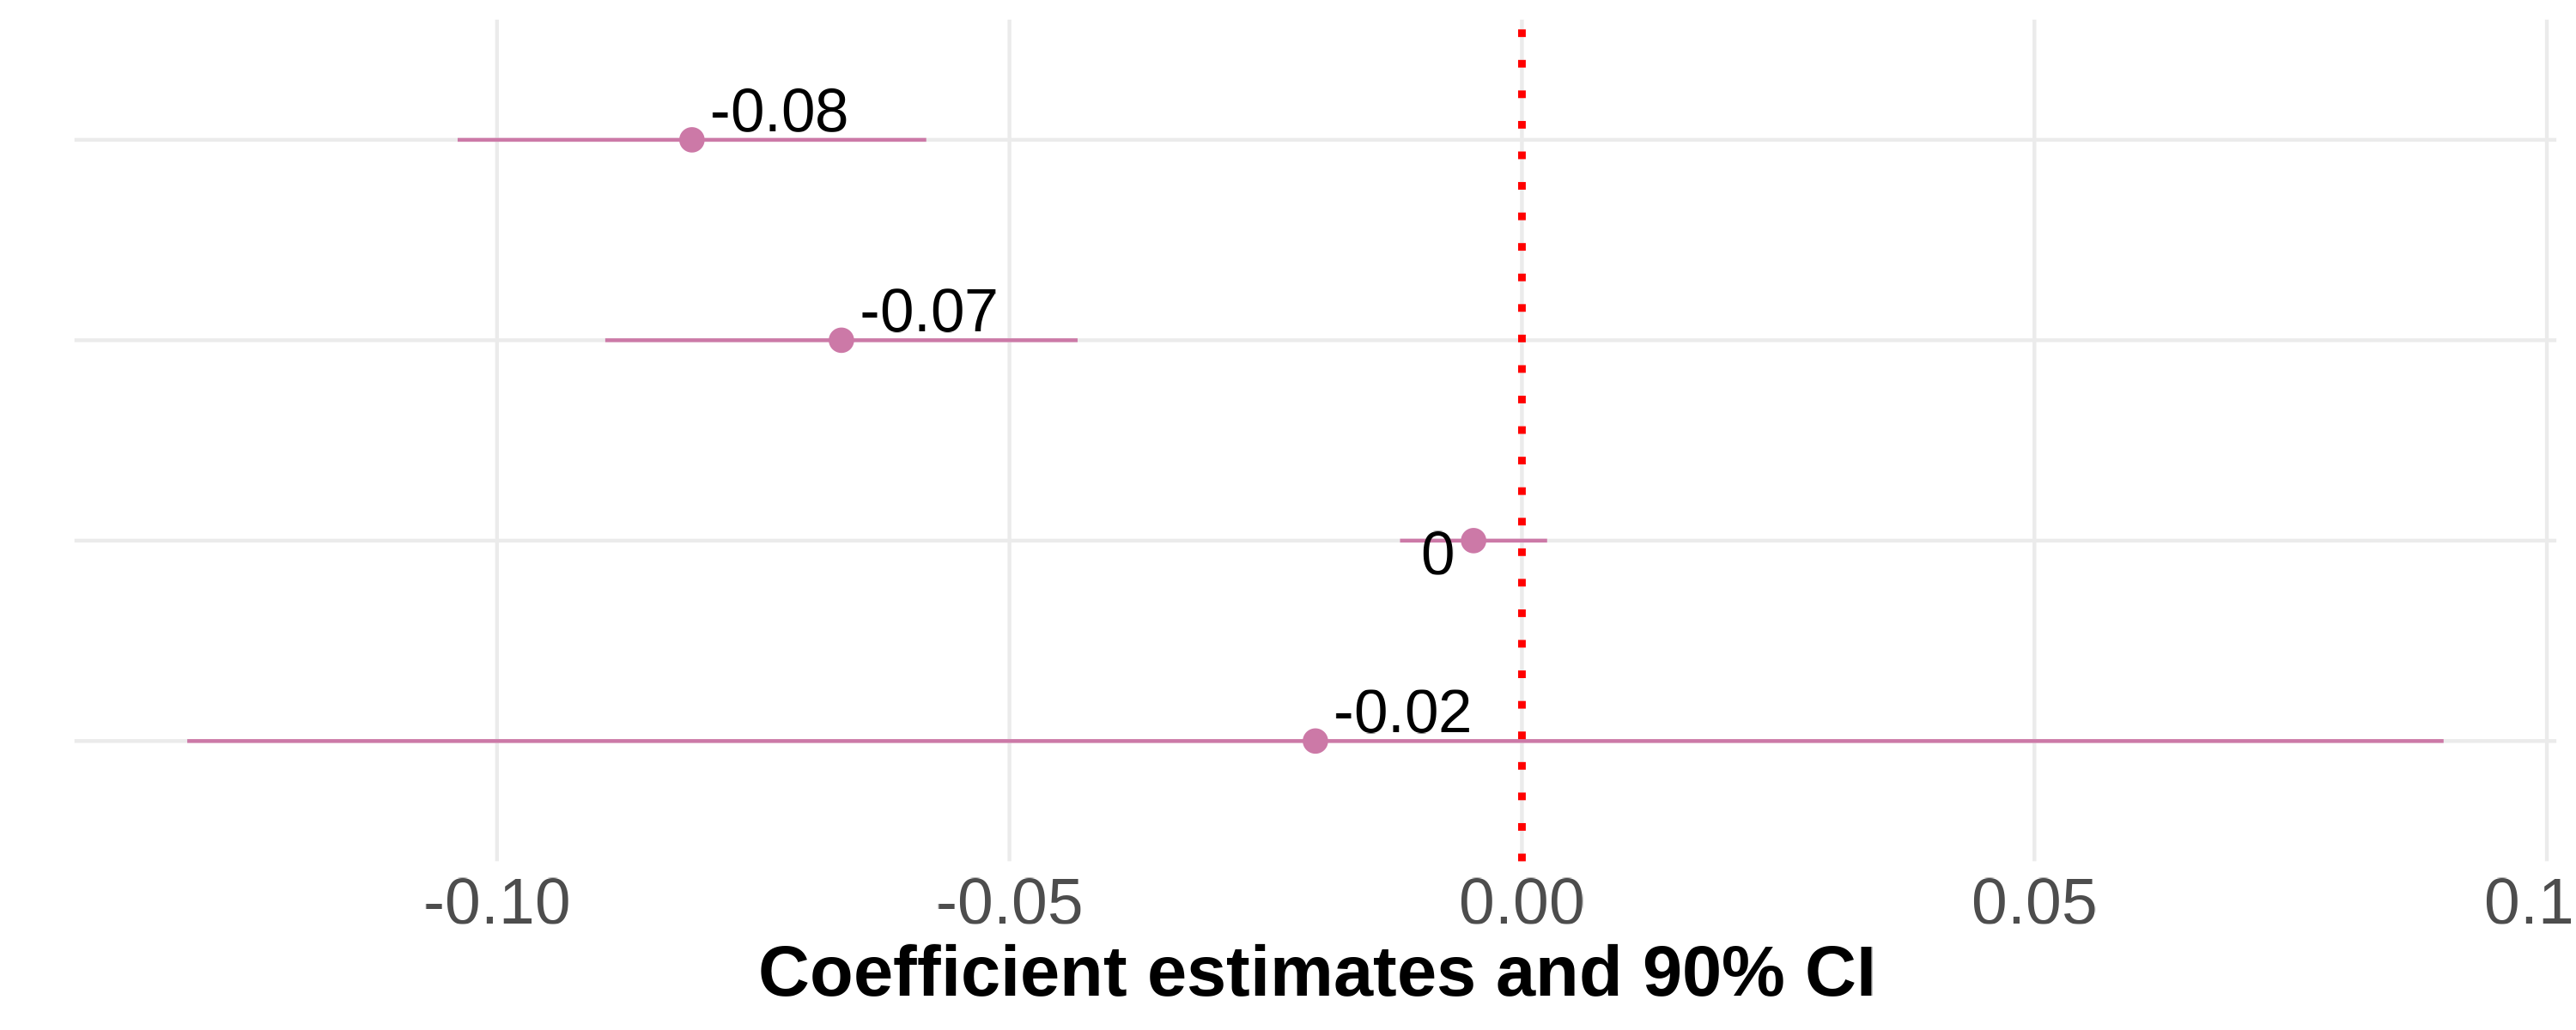
\includegraphics[width=.9\linewidth]{figure/skin-iat-regression-third-gen.png}
\end{subfigure}
\caption*{\footnotesize{I show four panels of estimating equation (\ref{eq:identity_reg_bias}). I include region $\times$ year fixed effects with controls for sex, quartic age, and parental education. The dependent variable is self-reported Asian identity and the independent variable is state-level bias. Each panel is the results from the same regression but on different samples that are divided by generation. Standard errors are clustered on the state level. The samples include first-, second-, and third-generation Asian children ages 17 and below who live in intact families. First-generation Asian immigrants are children that were born in a Asian country. Native-born second-generation Asian immigrants are children with at least one parent born in a Asian country. Finally, native-born third-generation Asian immigrants are children with native-born parents and at least one grandparent born in a Asian country.}}
\end{figure}
\end{center}

\pagebreak
\newpage

\begin{center}
\begin{figure}[!htb]
\centering
\caption{Relationship Between Self-Reported Asian Identity and Bias: By Parental Types}
\label{plot01-regression-byparent}
%First graph
\begin{subfigure}{.48\textwidth}
\caption{Second-Generation (All Parental Types)}
\centering
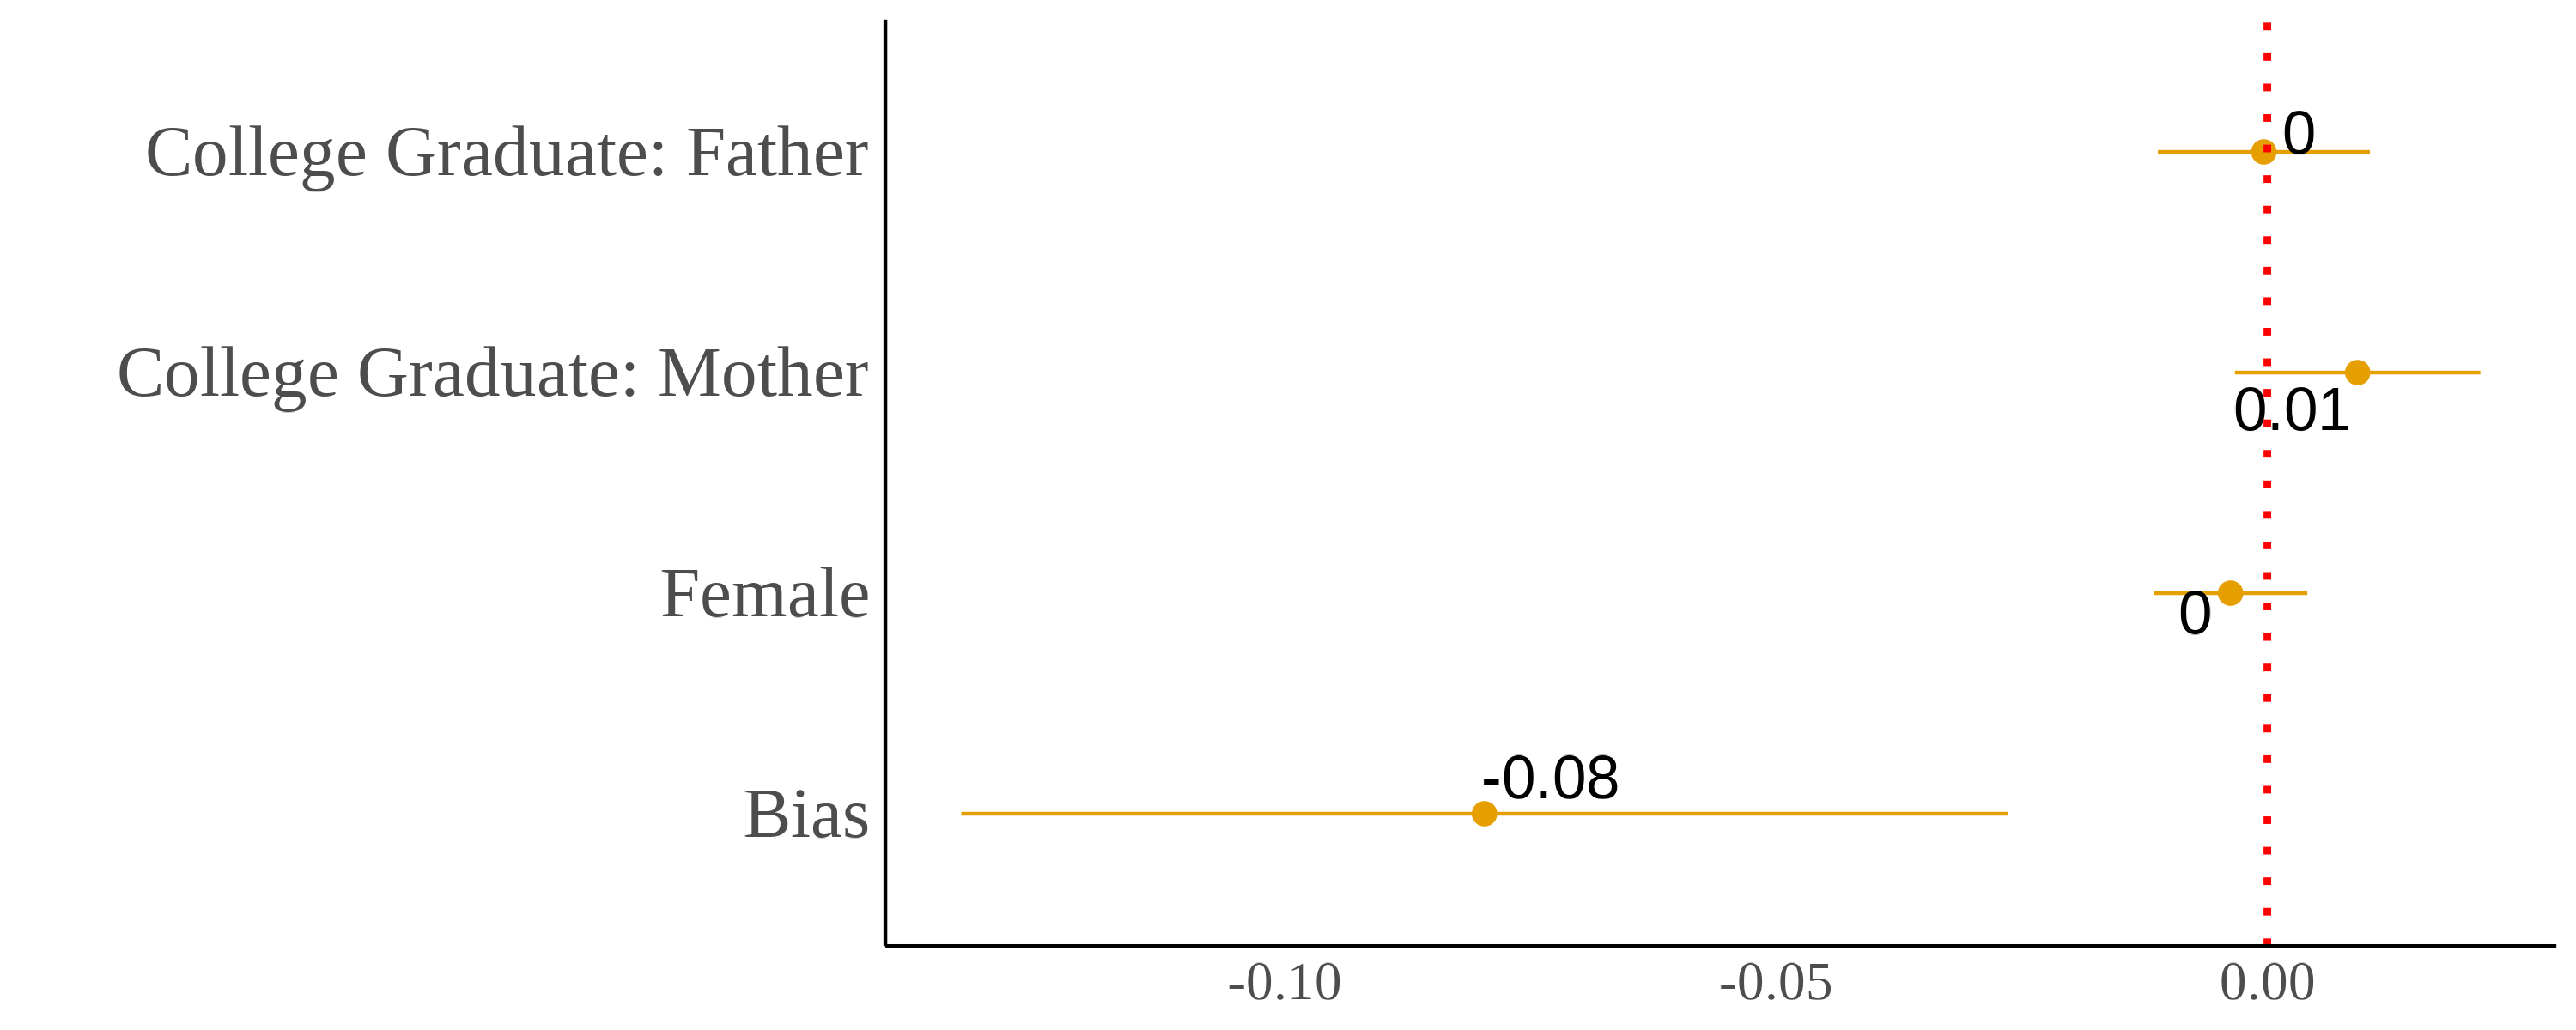
\includegraphics[width=.9\linewidth]{figure/by-parents-regs-all.png}
\end{subfigure}
\centering
%Second graph
\begin{subfigure}{.48\textwidth}
\caption{Asian Fathers-Asian Mothers}
\centering
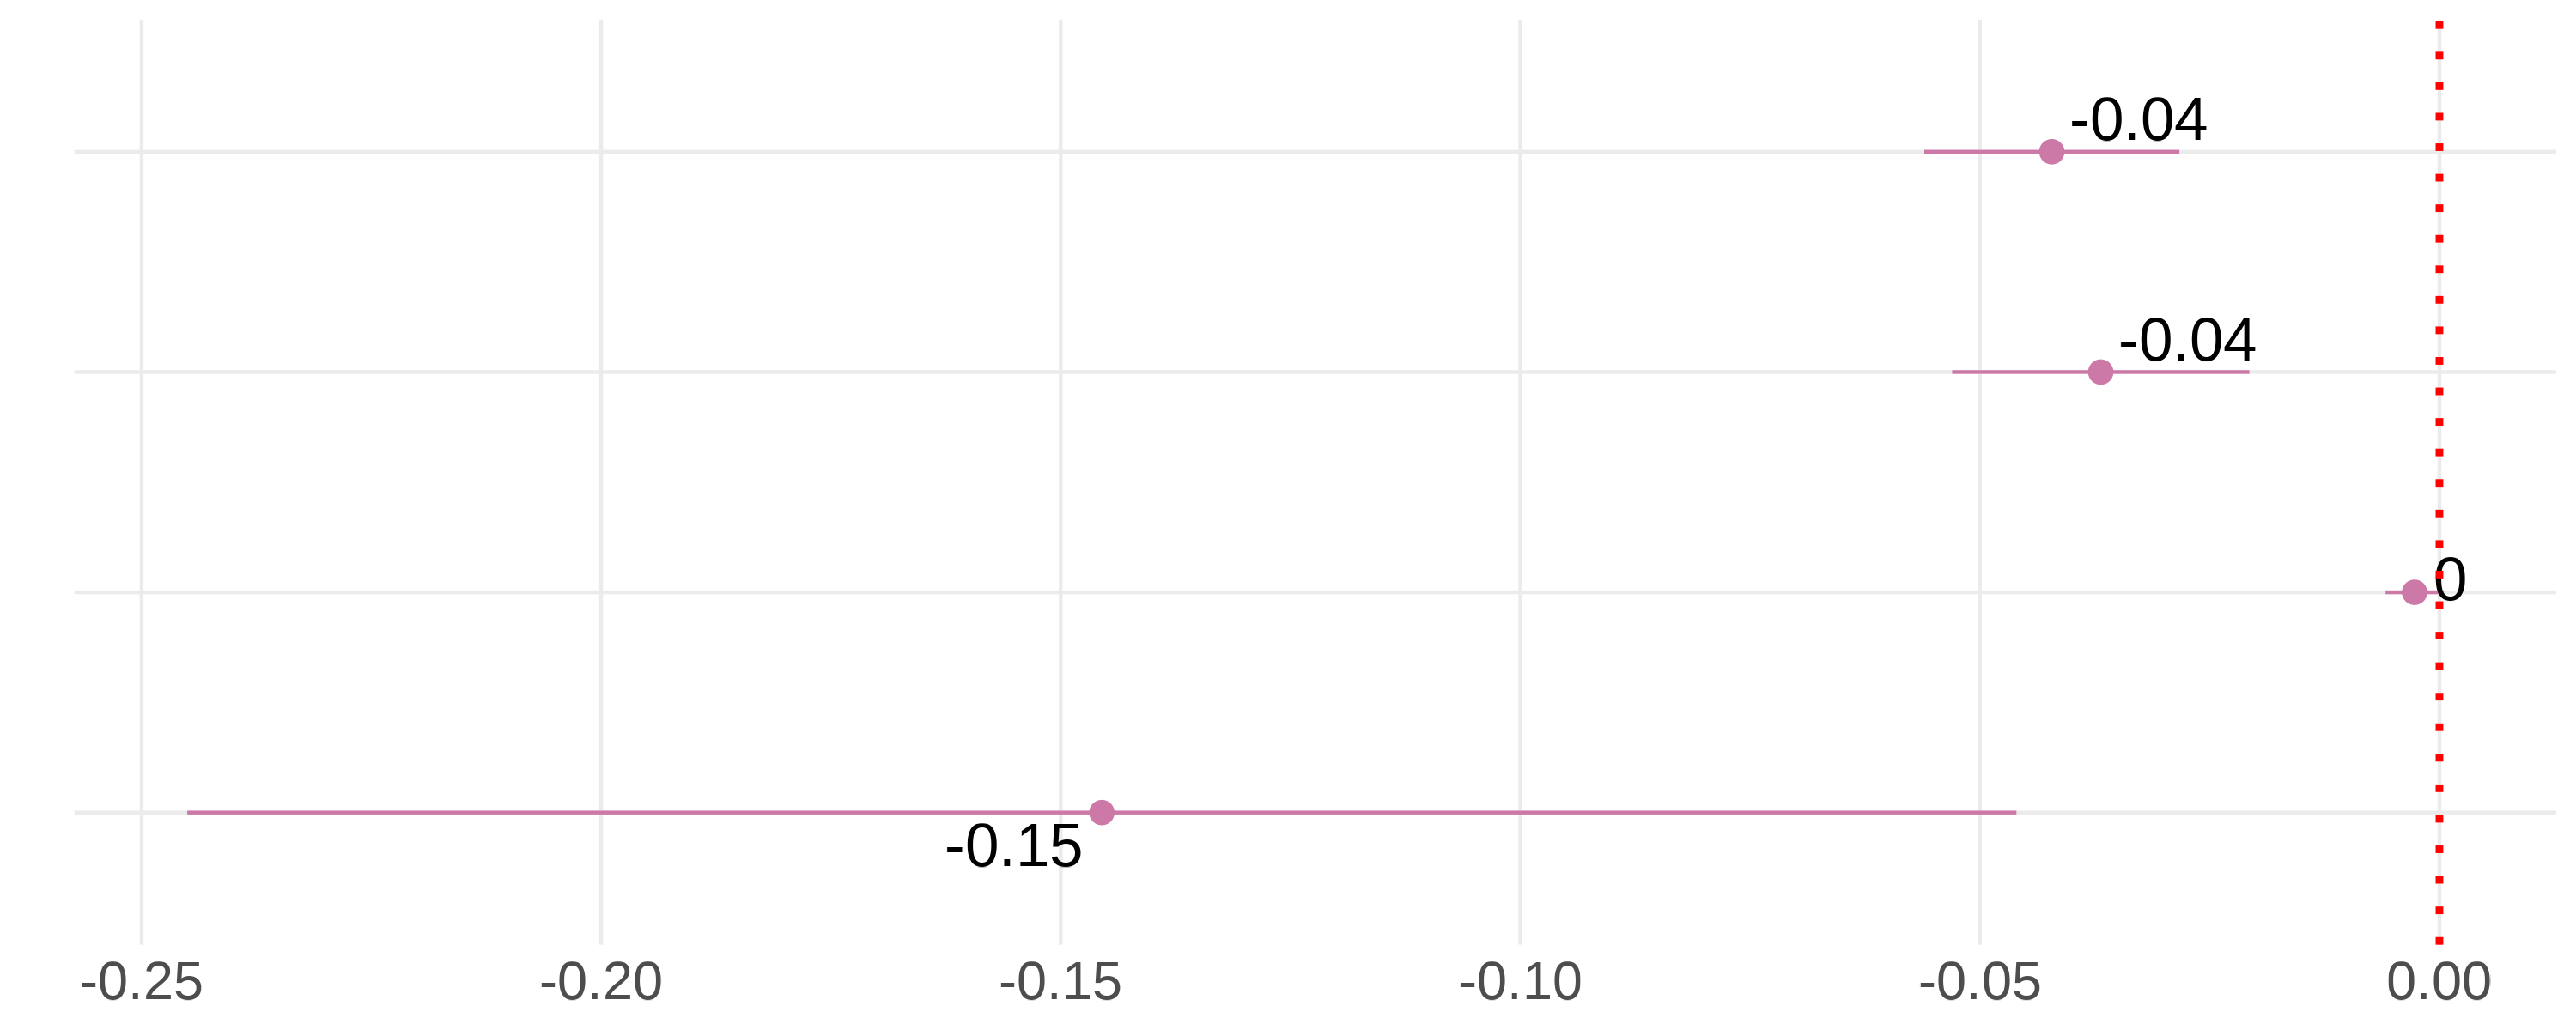
\includegraphics[width=.9\linewidth]{figure/by-parents-regs-hh.png}
\end{subfigure}
%Third Graph
\begin{subfigure}{.48\textwidth}
\caption{Asian Fathers-White Mothers}
\centering
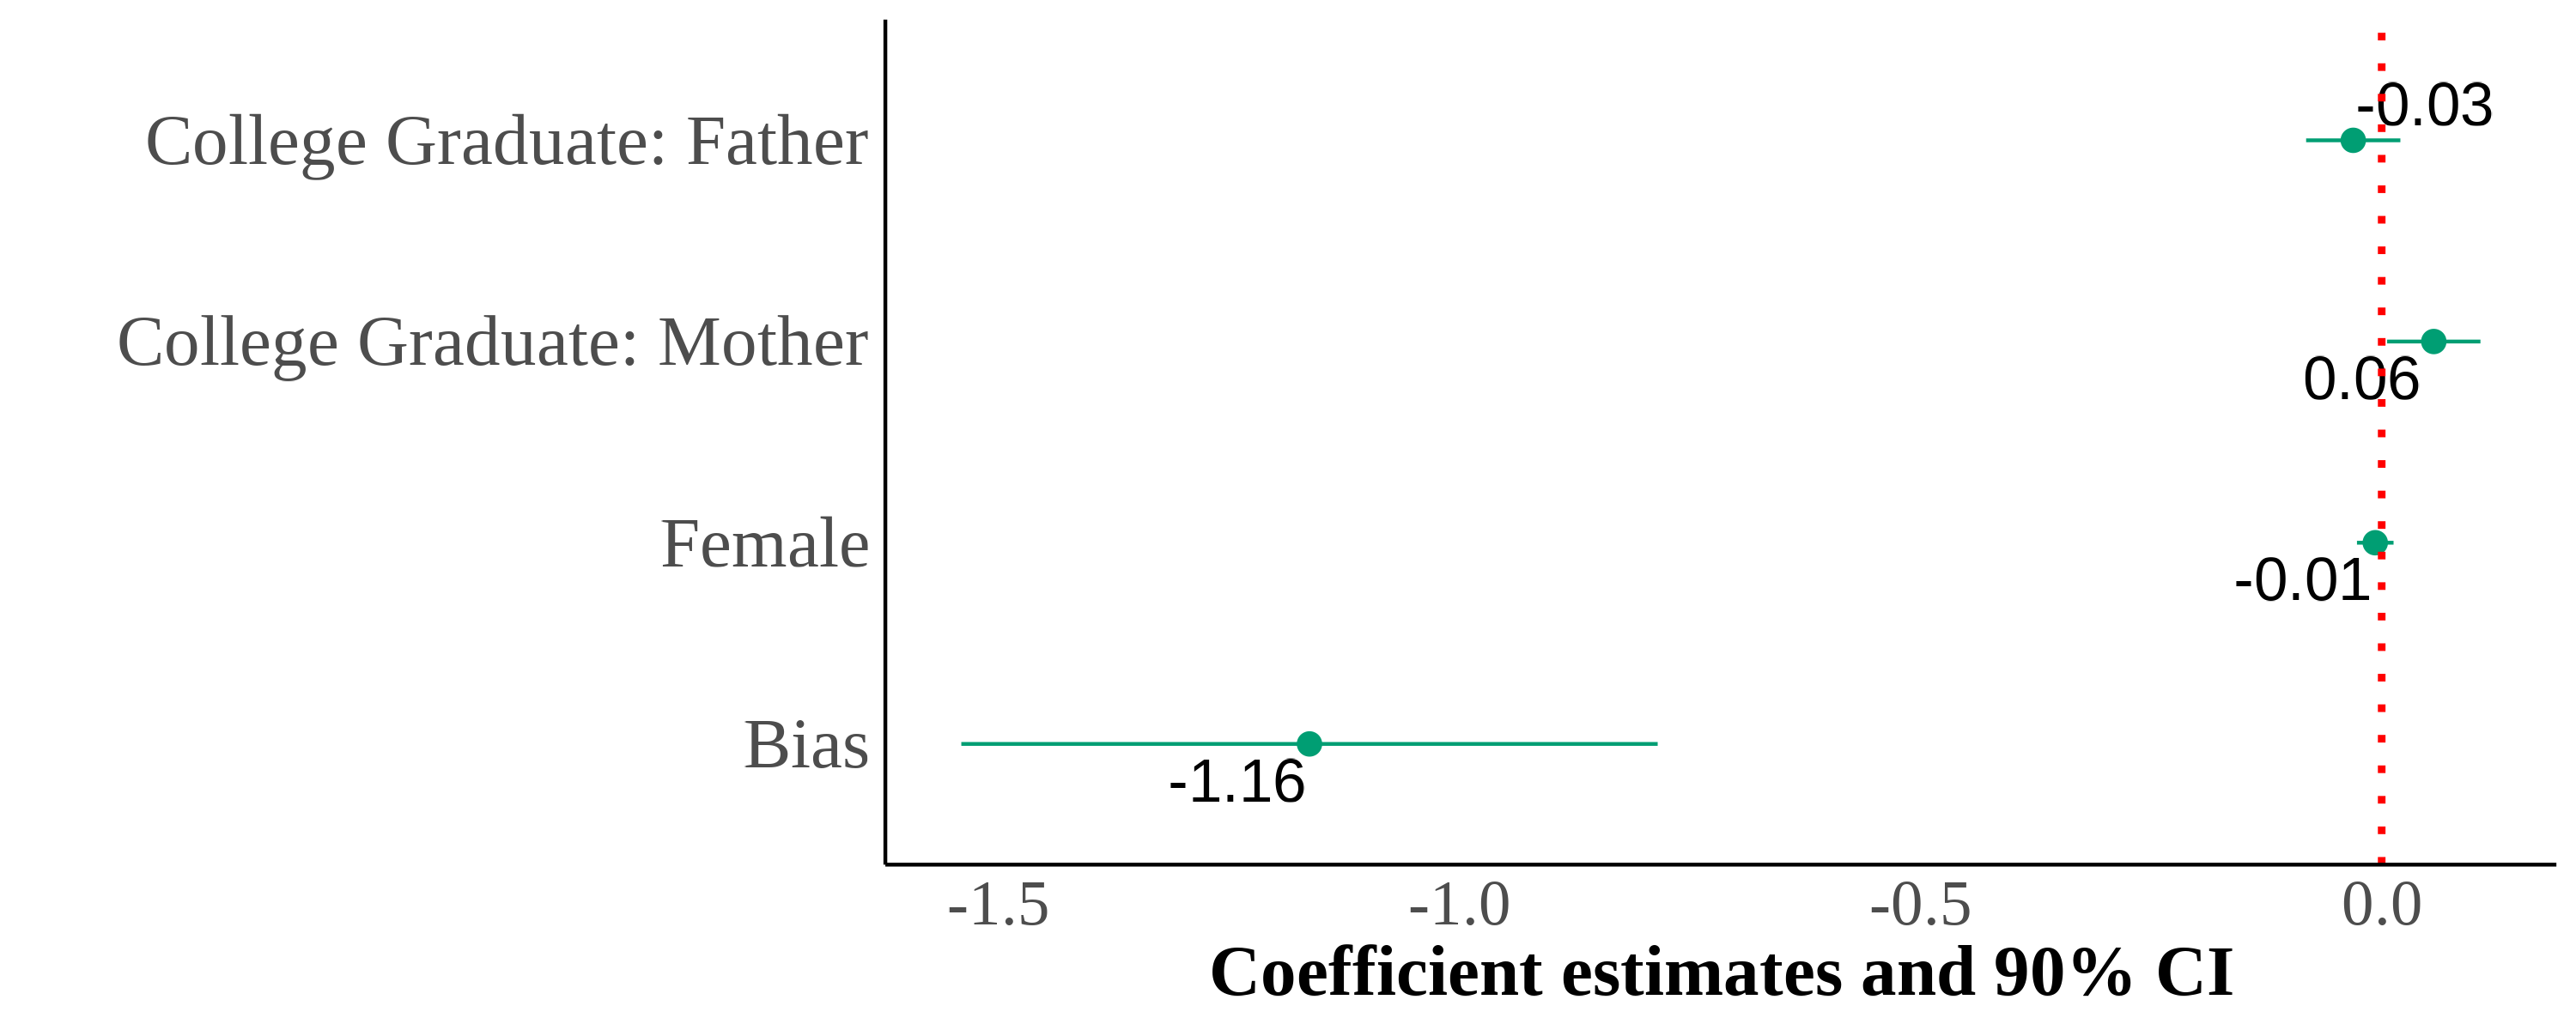
\includegraphics[width=.9\linewidth]{figure/by-parents-regs-hw.png}
\end{subfigure}
%Fourth Graph
\begin{subfigure}{.48\textwidth}
\caption{White Fathers-Asian Mothers}
\centering
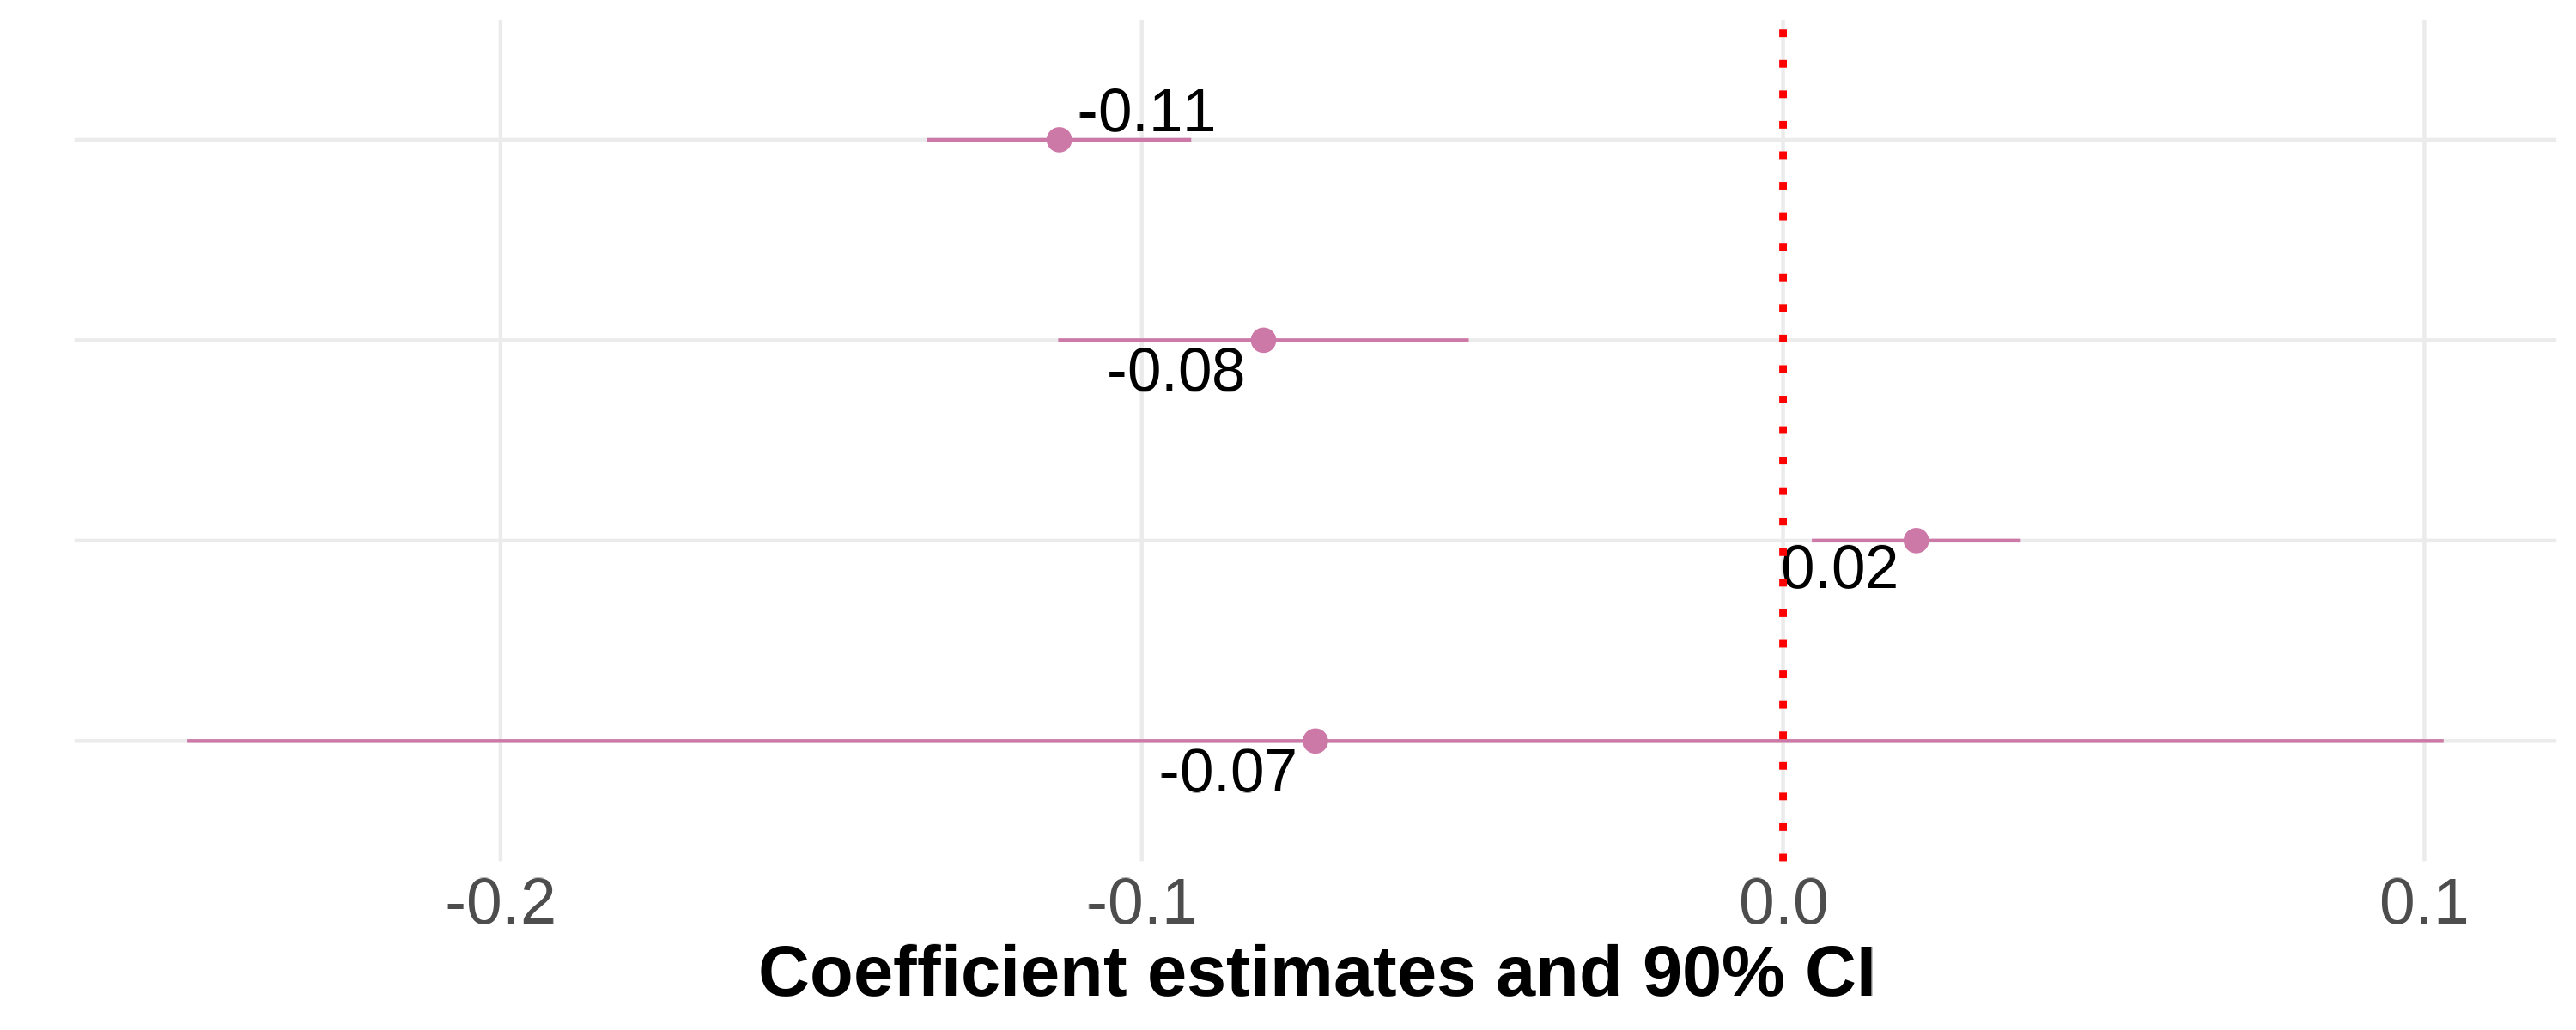
\includegraphics[width=.9\linewidth]{figure/by-parents-regs-wh.png}
\end{subfigure}
\caption*{\footnotesize{I show four panels of estimating equation (\ref{eq:identity_reg_bias}). I include region $\times$ year fixed effects with controls for sex, quartic age, and parental education. The dependent variable is self-reported Asian identity and the independent variable is state-level bias. Each panel results from the same regression but on different samples divided by parental types. Standard errors are clustered on the state level. The samples include second-generation Asian children ages 17 and below who live in intact families. Native-born second-generation Asian immigrant children with at least one parent born in a Spanish-speaking country.}}
\end{figure}
\end{center}

\pagebreak
\newpage

\begin{table}[H]

\caption{Relationship Between Bias and Self-Reported Hispanic identity Among Third-Generation Hispanic Immigrants: By Grandparental Type \label{regtab-bygrandparents}}
\centering
\resizebox{\linewidth}{!}{
\begin{threeparttable}
\begin{tabular}[t]{lcccc}
\toprule
\multicolumn{1}{c}{ } & \multicolumn{4}{c}{Number of Hispanic Grandparents} \\
\cmidrule(l{3pt}r{3pt}){2-5}
  & \specialcell{(1) \\ One} & \specialcell{(2) \\ Two} & \specialcell{(3) \\ Three} & \specialcell{(4) \\ Four}\\
\midrule
Bias & -0.04 & 0.03 & 0.19 & -0.14*\\
 & (0.11) & (0.09) & (0.26) & (0.07)\\
Female & -0.01 & 0.00 & -0.01 & 0.00\\
 & (0.01) & (0.01) & (0.01) & (0.01)\\
College Graduate: Mother & -0.11*** & -0.07*** & 0.02 & -0.02\\
 & (0.03) & (0.02) & (0.02) & (0.01)\\
College Graduate: Father & -0.11*** & -0.08*** & 0.02 & -0.03*\\
 & (0.03) & (0.01) & (0.01) & (0.01)\\
\midrule
Observations & 55,051 & 74,100 & 12,194 & 57,646\\
Year $\times$ Region FE & X & X & X & X\\
\bottomrule
\multicolumn{5}{l}{\rule{0pt}{1em}* p $<$ 0.1, ** p $<$ 0.05, *** p $<$ 0.01}\\
\end{tabular}
\begin{tablenotes}
\small
\item[1] \footnotesize{Each column is an estimation of equation (\ref{eq:identity_reg_bias}) restricted to third-generation Hispanic immigrants by 
                      number of Hispanic grandparents with region × year fixed effects. 
                      I include controls for sex, quartic age, fraction of Hispanics in a state, and parental education.
                      Standard errors are clustered on the state level.}
\item[2] \footnotesize{The samples include third-generation Hispanic children ages 17 and below who live in intact families. 
                      Native-born third-generation Hispanic 
                      immigrant children with at least one grandparent born in a Spanish-speaking 
                      country.}
\item[3] \footnotesize{Data source is the 2004-2021 Current Population Survey.}
\end{tablenotes}
\end{threeparttable}}
\end{table}


\pagebreak
\newpage

\begin{table}[H]
\centering\centering
\caption{Relationship Between Bias and Interethnic Marriages \label{regtab-logit-02}}
\centering
\begin{threeparttable}
\begin{tabular}[t]{lccc}
\toprule
\multicolumn{2}{c}{ } & \multicolumn{1}{c}{Asian Men} & \multicolumn{1}{c}{Asian Women} \\
\cmidrule(l{3pt}r{3pt}){3-3} \cmidrule(l{3pt}r{3pt}){4-4}
  & \specialcell{(1) \\ Interethnic} & \specialcell{(2) \\ Interethnic} & \specialcell{(3) \\ Interethnic}\\
\midrule
Bias & $0.04$*** & $-0.01$ & $0.03$**\\
 & ($0.01$) & ($0.01$) & ($0.01$)\\
College Graduate: Wife & $0.04$*** & $0.04$*** & $0.05$***\\
 & ($0.00$) & ($0.01$) & \vphantom{1} ($0.00$)\\
College Graduate: Husband & $-0.01$* & $-0.01$ & $-0.02$***\\
 & ($0.00$) & ($0.01$) & ($0.00$)\\
\midrule
Observations & $69,800$ & $52,103$ & $60,214$\\
Year $\times$ Region FE & X & X & X\\
\bottomrule
\multicolumn{4}{l}{\rule{0pt}{1em}* p $<$ 0.1, ** p $<$ 0.05, *** p $<$ 0.01}\\
\end{tabular}
\begin{tablenotes}
\small
\item[1] \footnotesize{This is the result to estimating (\ref{eq:inter-interethnic}) as a
                      linear probability model.}
\item[2] \footnotesize{I include controls for partners' sex, age, education, 
                      and years since immigrating to the United States.
                      Standard errors are clustered on the household level.}
\item[3] \footnotesize{Data source is the 2004-2020 Current Population Survey Data.}
\end{tablenotes}
\end{threeparttable}
\end{table}


\pagebreak
\newpage

\begin{table}[H]
\centering\centering
\caption{Main Effect of Proxy on Second-Generation's Asian Self-identification \label{tab:hispbyproxy}}
\centering
\fontsize{12}{14}\selectfont
\begin{tabular}[c]{>{}lllll}
\toprule
Parents Type & All & Asian-Asian & Asian-White & White-Asian\\
\midrule
\textbf{Proxy:} &  &  &  & \\
\hspace{1em}\textbf{Mother} & 0.72 & 0.97 & 0.37 & 0.3\\
\hspace{1em}\textbf{Father} & 0.72 & 0.97 & 0.39 & 0.29\\
\hspace{1em}\textbf{Self} & 0.87 & 0.97 & 0.23 & 0.31\\
\hspace{1em}\textbf{Others} & 0.88 & 0.96 & 0.6 & 0.54\\
\bottomrule
\end{tabular}
\end{table}


\pagebreak
\newpage


\begin{table}[H]
\centering\centering
\caption{Main Effect of Proxy on Second-Generation's Asian Self-identification \label{tab:hispbyproxy}}
\centering
\fontsize{12}{14}\selectfont
\begin{tabular}[c]{>{}lllll}
\toprule
Parents Type & All & Asian-Asian & Asian-White & White-Asian\\
\midrule
\textbf{Proxy:} &  &  &  & \\
\hspace{1em}\textbf{Mother} & 0.72 & 0.97 & 0.37 & 0.3\\
\hspace{1em}\textbf{Father} & 0.72 & 0.97 & 0.39 & 0.29\\
\hspace{1em}\textbf{Self} & 0.87 & 0.97 & 0.23 & 0.31\\
\hspace{1em}\textbf{Others} & 0.88 & 0.96 & 0.6 & 0.54\\
\bottomrule
\end{tabular}
\end{table}


\clearpage
